%%%%%%%%%%%%%%%%%%%%%%%%%%%%%%%%%%%%%%%%%
% Masters/Doctoral Thesis 
% LaTeX Template
% Version 2.5 (27/8/17)
%
% This template was downloaded from:
% http://www.LaTeXTemplates.com
%
% Version 2.x major modifications by:
% Vel (vel@latextemplates.com)
%
% This template is based on a template by:
% Steve Gunn (http://users.ecs.soton.ac.uk/srg/softwaretools/document/templates/)
% Sunil Patel (http://www.sunilpatel.co.uk/thesis-template/)
%
% Template license:
% CC BY-NC-SA 3.0 (http://creativecommons.org/licenses/by-nc-sa/3.0/)
%
%%%%%%%%%%%%%%%%%%%%%%%%%%%%%%%%%%%%%%%%%

%----------------------------------------------------------------------------------------
%	PACKAGES AND OTHER DOCUMENT CONFIGURATIONS
%----------------------------------------------------------------------------------------

\documentclass[
11pt, % The default document font size, options: 10pt, 11pt, 12pt
oneside, % Two side (alternating margins) for binding by default, uncomment to switch to one side
english, % ngerman for German
singlespacing, % Single line spacing, alternatives: onehalfspacing or doublespacing
%draft, % Uncomment to enable draft mode (no pictures, no links, overfull hboxes indicated)
%nolistspacing, % If the document is onehalfspacing or doublespacing, uncomment this to set spacing in lists to single
%liststotoc, % Uncomment to add the list of figures/tables/etc to the table of contents
%toctotoc, % Uncomment to add the main table of contents to the table of contents
%parskip, % Uncomment to add space between paragraphs
%nohyperref, % Uncomment to not load the hyperref package
headsepline, % Uncomment to get a line under the header
%chapterinoneline, % Uncomment to place the chapter title next to the number on one line
%consistentlayout, % Uncomment to change the layout of the declaration, abstract and acknowledgements pages to match the default layout
]{MastersDoctoralThesis} % The class file specifying the document structure

\usepackage[utf8]{inputenc} % Required for inputting international characters
\usepackage{lmodern,textcomp}
\usepackage[T1]{fontenc} % Output font encoding for international characters
\usepackage{pdflscape}

\usepackage{mathpazo} % Use the Palatino font by default

\usepackage[backend=bibtex]{biblatex} % Use the bibtex backend with the authoryear citation style (which resembles APA)

\addbibresource{main.bib} % The filename of the bibliography

\usepackage[autostyle=true]{csquotes} % Required to generate language-dependent quotes in the bibliography

\usepackage[firstpage]{draftwatermark}
\SetWatermarkText{\shortstack{
		Document \\[1em] in progress 
	}}
\SetWatermarkScale{1}

\usepackage{amssymb}

%----------------------------------------------------------------------------------------
%	MARGIN SETTINGS
%----------------------------------------------------------------------------------------

\geometry{
	paper=a4paper, % Change to letterpaper for US letter
	inner=2.5cm, % Inner margin
	outer=3.8cm, % Outer margin
	bindingoffset=.5cm, % Binding offset
	top=1.5cm, % Top margin
	bottom=1.5cm, % Bottom margin
	%showframe, % Uncomment to show how the type block is set on the page
}

%----------------------------------------------------------------------------------------
%	THESIS INFORMATION
%----------------------------------------------------------------------------------------

\thesistitle{\projectTitle} % Your thesis title, this is used in the title and abstract, print it elsewhere with \ttitle
\supervisor{Dr. Jordi \textsc{Cortadella}} % Your supervisor's name, this is used in the title page, print it elsewhere with \supname
\examiner{} % Your examiner's name, this is not currently used anywhere in the template, print it elsewhere with \examname
\degree{Computer Science Degree} % Your degree name, this is used in the title page and abstract, print it elsewhere with \degreename
\author{Marc \textsc{Benedí}} % Your name, this is used in the title page and abstract, print it elsewhere with \authorname
\addresses{} % Your address, this is not currently used anywhere in the template, print it elsewhere with \addressname

\subject{} % Your subject area, this is not currently used anywhere in the template, print it elsewhere with \subjectname
\keywords{} % Keywords for your thesis, this is not currently used anywhere in the template, print it elsewhere with \keywordnames
\university{\href{https://www.upc.edu/ca}{Universitat Politècnica de Catalunya}} % Your university's name and URL, this is used in the title page and abstract, print it elsewhere with \univname
\department{\href{https://www.fib.upc.edu/ca/recerca/departaments/ciencies-de-la-computacio}{Department of Computer Science}} % Your department's name and URL, this is used in the title page and abstract, print it elsewhere with \deptname
\group{\href{}{}} % Your research group's name and URL, this is used in the title page, print it elsewhere with \groupname
\faculty{\href{https://www.google.co.uk/search?ei=y0GXWteBJsXSwQLJ8IGIDA&q=fib&oq=fib&gs_l=psy-ab.3..35i39k1l2j0i67k1j0l7.1898.2078.0.2162.3.3.0.0.0.0.92.172.2.2.0....0...1.1.64.psy-ab..1.2.172....0.Ha_7J3E1vcI}{Facultat Informàtica de Barcelona}} % Your faculty's name and URL, this is used in the title page and abstract, print it elsewhere with \facname

\newcommand{\projectTitle}{Design of an environment for solving pseudo-boolean optimization problems}
\newcommand{\courseName}{Dissertation}
\newcommand{\city}{Geneva, Switzerland}

\AtBeginDocument{
\hypersetup{pdftitle=\ttitle} % Set the PDF's title to your title
\hypersetup{pdfauthor=\authorname} % Set the PDF's author to your name
\hypersetup{pdfkeywords=\keywordnames} % Set the PDF's keywords to your keywords
}

\begin{document}

\frontmatter % Use roman page numbering style (i, ii, iii, iv...) for the pre-content pages

\pagestyle{plain} % Default to the plain heading style until the thesis style is called for the body content

%----------------------------------------------------------------------------------------
%	TITLE PAGE
%----------------------------------------------------------------------------------------

\begin{titlepage}
\begin{center}

\vspace*{.06\textheight}
{\scshape\LARGE \univname\par}\vspace{1.5cm} % University name
\textsc{\Large \ttitle}\\[0.5cm] % Thesis type

\HRule \\[0.4cm] % Horizontal line
{\huge \bfseries \projectTitle\par}\vspace{0.4cm} % Thesis title
\HRule \\[1.5cm] % Horizontal line
 
\begin{minipage}[t]{0.4\textwidth}
\begin{flushleft} \large
\emph{Author:}\\
\href{http://marcb.pro}{\authorname} % Author name - remove the \href bracket to remove the link
\end{flushleft}
\end{minipage}
\begin{minipage}[t]{0.4\textwidth}
\begin{flushright} \large
\emph{Supervisor:} \\
\href{https://www.cs.upc.edu/~jordicf/}{\supname} % Supervisor name - remove the \href bracket to remove the link  
\end{flushright}
\end{minipage}\\[3cm]
 
\vfill

\large \textit{ }\\[0.3cm] % University requirement text
\textit{ }\\[0.4cm]
%\groupname\\\deptname\\[2cm] % Research group name and department name
\courseName\\[2cm]
\vfill

{\large \today \\ \city}\\[4cm] % Date
%
\includegraphics{UPCLogo.png} % University/department logo - uncomment to place it
 
\vfill
\end{center}
\end{titlepage}

%----------------------------------------------------------------------------------------
%	ABSTRACT PAGE
%----------------------------------------------------------------------------------------

\begin{abstract}
	\addchaptertocentry{\abstractname} % Add the abstract to the table of contents
    This dissertation addresses several approaches with the common goal of reducing the time required to solve Pseudo-Boolean minimisation problems.  A C++ library has been developed which allows representing Pseudo-Boolean minimisation problems smoothly. The problem entered for the user is encoded into a CNF using PBLib. Two different algorithms are used to search for the minimum value for the cost function: Linear search and Binary search. Finally, two timeout strategies are implemented: General timeout and Simple timeout which stops the solver and returns the last minimum value found. 
	
\end{abstract}

%----------------------------------------------------------------------------------------
%	GLOSSARY
%----------------------------------------------------------------------------------------

\begin{abbreviations}{ll} % Include a list of abbreviations (a table of two columns)
	
	\textbf{Abbreviation} & Description of the abbreviation\\
	
	\textbf{} & \\
	\textbf{BF} & \textbf{B}oolean \textbf{F}ormula\\
	\textbf{CNF} & \textbf{C}onjunctive \textbf{N}ormal \textbf{F}orm \\
	\textbf{DNF} & \textbf{D}isjunctive \textbf{N}ormal \textbf{F}orm\\
	\textbf{PB} & \textbf{P}seudo-\textbf{B}oolean\\
	\textbf{PBF} & \textbf{P}seudo-\textbf{B}oolean \textbf{F}ormula\\
	\textbf{SAT} & Boolean \textbf{sat}isfiability problem\\
	\textbf{PB-Min} & \textbf{P}seudo-\textbf{B}oolean \textbf{Min}imisation\\
	\textbf{BF} & \textbf{B}oolean \textbf{F}ormula \\
	\textbf{NP} & \textbf{N}ondeterministic \textbf{P}olynomial time\\
	\textbf{BDD} & \textbf{B}inary \textbf{D}ecision \textbf{D}iagram\\
	\textbf{AI} & \textbf{A}rtificial \textbf{I}ntelligence\\
	\textbf{TDD} & \textbf{T}est-\textbf{D}riven \textbf{D}evelopment\\
\end{abbreviations}

%----------------------------------------------------------------------------------------
%	LIST OF CONTENTS/FIGURES/TABLES PAGES
%----------------------------------------------------------------------------------------

\tableofcontents % Prints the main table of contents

\listoffigures % Prints the list of figures

\listoftables % Prints the list of tables

%----------------------------------------------------------------------------------------
%	THESIS CONTENT - CHAPTERS
%----------------------------------------------------------------------------------------

\mainmatter % Begin numeric (1,2,3...) page numbering

\pagestyle{thesis} % Return the page headers back to the "thesis" style

% Include the chapters of the thesis as separate files from the Chapters folder
% Uncomment the lines as you write the chapters

\chapter{Introduction and Context}
\label{Chapter1}

\section{Introduction}

\section{Context}

Before explaining the main problem which this project is about, \emph{Pseudo-Boolean Minimization}, it necessary to do a quick introduction to a much wider topic.\\

\textbf{Boolean satisfiability problems} \textit{(SAT from now on)} is the problem of finding a model\footnote{An interpretation which satisfies the formula.} for a \emph{Boolean Formula} (BF from now on). In other words, it is the result of evaluating the \emph{BF} after replacing its variables for \emph{true} or \emph{false}. 
\\
\emph{SAT} is widely used in Computer Science because it was the first problem proved to be NP-Complete\cite{Cook1971}\footnote{NP and NP-Hard.} which allowed a lot of NP\footnote{Nondeterministic polynomial time.} problems be reduced to it.

\subsubsection{What is a Pseudo-Boolean Formula?}
In propositional logic, a \emph{BF} is defined as following\cite{Lpo}:\\
Let $P$ be a set of predicate symbols like $p,q,r,...$
\begin{itemize}
	\item All predicate symbol of $P$ is a formula.
	\item If $F$ and $G$ are formulae, then $(F \land G)$ and $(F \lor G)$ are formulae too.
	\item If $F$ is a formula, then $(\neg F)$ is a formula.
	\item Nothing else is a formula.
\end{itemize}
This representation has some limitations because it can only express properties which are \emph{true} or \emph{false}.\\

\emph{Pseudo-Boolean Formulas} are functions of the form $f:B^n \rightarrow \mathbb{R}$. For example, the following formula is a \emph{Pseudo-Boolean Formula} (PBF from now on): $3x+5y$. Therefore, \emph{BF} are a special case of \emph{PBF} where the domain is $d=\{0,1\}$.\\

%TODO: potser explicar que son cardinality constraints


\subsubsection{Pseudo-Boolean formulae minimization}
\emph{PBF minimization} is a well known NP-Hard\footnote{NP-Hard: at least as hard as the hardest problems in NP \href{https://en.wikipedia.org/wiki/NP-hardness}{(more)}} problem. \\
It does the following:\\
Given some \emph{PB Constraints} of the form $\sum_{i=1}^{n} x_{i}w_{i} \leq k$, where $w_{i},k \in \mathbb{I}$ and $x_{i} \in \{0,1\}$, and a cost function , the goal is minimize it  $min(a_{1}x{1} + ... + a_{n}x_{n})$ in a way that all the restrictions are satisfied.\\

There is a big research in this field, more specifically in encoding \emph{PBF} into \emph{CNF}. In this paper, Hölldobler, Manthey, Steinke\cite{Holldobler}, some relevant \emph{PBF} into \emph{SAT} encodings are explained and a new one is proposed. One of the authors of this paper, Steinke, is also the author of \emph{PBLib}.  

\section{Background}

During the past semester (Q1 2017/2018), under the supervision of \href{https://www.cs.upc.edu/~jordicf/}{Dr. Jordi Cortadella}, I had been developing a C++ library.\\
This tool allows the users to represent \emph{BF} in a C++ program in an intuitive way, do operations between them and convert them into \emph{Binary Decision Diagrams} (BDD from now on). However, the main functionality of this library is the conversion from a \emph{BF} to \emph{CNF}.  \\
As previously explained, \emph{CNF} is a particular type of a \emph{BF}, a conjunction of disjunctions. \emph{CNF} is an important format because it is the standard input for \emph{SAT Solvers}\ref{A.1}.\\
As shown in this paper, \emph{Mitchell, Selman, and Levesque\cite{Mitchell}}, there is a correlation between the number of variables, the number of clauses and the hardness of solving the \emph{CNF}.
\begin{center}
	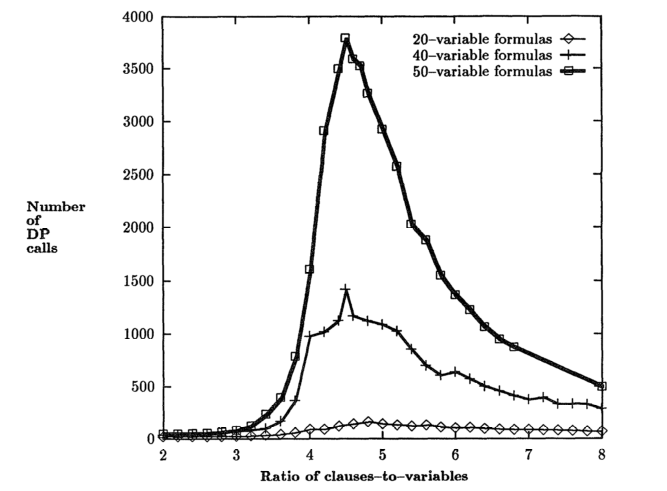
\includegraphics[width=1\textwidth]{Figures/GraphMitchellSelmanLevesque.png}
	\captionof{figure}{Median number of recursive DP calls for Random 3-SAT formulas, as a function of the ratio of clauses-to-variables. \\Extracted from Mitchell, Selman, and Levesque\cite{Mitchell}}
\end{center}
Therefore, an improvement of the input \emph{CNF} of the \emph{SAT Solver} can reduce a lot the hardness of the problem. \\
This is the main goal of the library, try to reduce the size of the final \emph{CNF} resulting from applying different converting methods on the original BF.

\section{State-of-the-art}

In this section, previous projects are discussed. \\
The first one is \href{http://tools.computational-logic.org/content/pblib.php}{PBLib}. PBLib is a C++ toolkit for encoding \emph{PB Constraints} into \emph{CNF}.\\
As explained in \emph{Steinke}\cite{Steinke2015}, PBLib implements a lot of encodings:
\begin{center}
	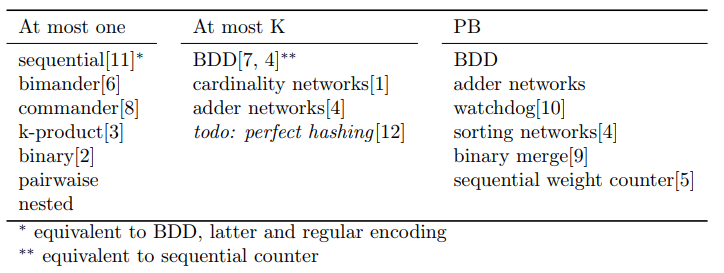
\includegraphics[width=1\textwidth]{Figures/PBLibEncodings.png}
	\captionof{figure}{PBLib implemented encodings\\Extracted from Steinke\cite{Steinke2015}}
\end{center}
PBLib does not only implement these encodings, the most interesting thing is that it can decide which encoder provides the most effective translation.\\
It is very hard to compete on this aspect against PBLib, but it is not very user-friendly. For this reason, on of the goals of this project is to add a layer between the user and PBLib to simplify how the user declares the \emph{PB Constraints}.\\\\

The second project we will talk about is the explained in the \emph{Background section}. This project adds a new encoding for \emph{BF} which can be extended to \emph{PB Constraints}. This encoding will be studied and if it achieves good metrics it will be implemented to \emph{PB Constraints}


\section{Motivations}

\href{https://www.fib.upc.edu/en/studies/bachelors-degrees/bachelor-degree-informatics-engineering/curriculum/syllabus/LI}{Informatics Logic} is taught in this\footnote{\href{https://www.fib.upc.edu/en/}{Facultat Informàtica de Barcelona}} faculty. In that course, I realized how important is \emph{logic} through its lecturer, \href{http://www.lsi.upc.es/~roberto/}{Dr. Robert Nieuwenhuis}, and its activities. \\

In the first coursework, we had to code a \emph{SAT Solver} which used \emph{Unit Propagation}.
%\ref{A.2}. 
With this activity, I comprehended how hard and substantial is the study of \emph{logic} and all its context. For example, how \emph{logic} is used in Artificial Intelligence and Planners.\\

When the time of deciding the \emph{TFG} arrived, I contacted my actual supervisor, \href{https://www.cs.upc.edu/~jordicf/}{Dr. Jordi Cortadella}, and he proposed me some topics and ideas. Finally, we agreed on doing this project. \\

The motivation for this project is trying to deepen into the topic and contribute on it.

\section{Stakeholders}

In this section, the Stakeholders of the project are defined. Stakeholders are entities which are affected, directly or indirectly, by the solution developed in this project. 
\subsection{Target audience}
This tools targets all the entities (researchers, companies, \ldots) which work with \emph{PB minimization} and use \emph{SAT Solvers}.
\subsection{Users}
The users will be C++ programmers due this tool is developed in this language.
\subsection{Beneficiaries}
All those entities which work with \emph{PB minimization}. For example AI, SAT Solvers, Planners, \ldots
\chapter{Project Scope}
\label{Chapter2}

\section{Project Formulation}

As mentioned before\ref{Chapter1}, this project is an extension of a previous C++ library. The main goal of this project is to improve the time required to solve \emph{minimisation} problems. To achieve this goal the following objectives have been established. 

\subsection{General objectives}

\subsubsection{Pseudo-Boolean minimization}
For the problems formed by some \emph{PB Constraints} $min(c_{1}x_{1}+c_{2}x_{2}+\ldots +c_{n}x_{n} \leq k)$ and a cost function , the goal is to find and assignment for $\{x_{1},x_{2},\ldots,x_{n}\}$ in a way that the cost function is minimised. $$min(a_{1}x{1} + ... + a_{n}x_{n})$$

Previously\ref{Chapter1}, it has been explained that this types of problems are \emph{NP-Hard}. This project will try to reduce the time to solve these problems through two approaches:
\begin{itemize}
	\item Binary search:\\
	Implement the well known \emph{Binary Search} algorithm to find the minimum value for the cost function.	
	\item Linear search:\\
	Some \emph{SAT Solvers} can learn and derive new restrictions from previous problems. To take advantage of this ability, it is necessary to implement a \emph{Linear Search} algorithm.
\end{itemize}

\subsubsection{Timeout}
For some problems, it is more important to find a solution before a deadline than finding the best possible solution. For instance, a delivery company must have all the routes planned for all trucks before the journey starts, therefore, they care more about having a solution than finding the best one.\\
For this, a \emph{Timeout strategy} will be implemented in case that a good enough solution has been found or the problem does not seem to have one. 
\subsubsection{Multi-threading (Optional)}
This tool will take advantage of multi-core processors trying to split the problem and solving each part separately.

\section{Scope}
\subsection{What and how?}

To achieve all the general objectives\ref{Chapter2} of the project the following stages have been established:
\begin{itemize}
	\item Analyze, refactor\footnote{Code refactoring is the process of restructuring existing computer code—changing the factoring—without changing its external behavior. \href{https://en.wikipedia.org/wiki/Code_refactoring}{(more)}} and test the existing code to have a solid base. 
	\item Add the functionality of representing \emph{PBF}.
	\item Study \href{http://tools.computational-logic.org/content/pblib.php}{PBLib} library to see which functionalities it has available to work with \emph{minimisation}.
	\item Implement \emph{minimisation} strategies.
	\item Study timeout strategies and implement them.
	\item Study and implement multithreading. (Optional)
\end{itemize}

\subsection{Possible obstacles}

In this section, the possible obstacles and its solutions are exposed.

\subsubsection{Base project}
The existing project \emph{Background section}\ref{Chapter1} has not been developed following an adequate methodology. This bad practice could be responsible for a poor code quality. Building on top of a program with this characteristics could have terrible consequences because it would produce a lot of bugs and malfunctions hard to solve in the future. \\
For this reason, it is better to improve the quality of the existing code because it will avoid problems in the future.

\subsubsection{Schedule}
Because this is a final degree project, the scope is limited, in this case until June of 2018. Considering the learning stage, analysis, requirements study, and other deviations which could appear, the time available to develop the project could be drastically reduced.  Moreover, this project will be developed in an Erasmus stay which makes more laborious the planning. 
For these reasons, a good and realistic planning are key steps to take advantage of time and reduce contingencies. 

\subsubsection{PBLib}
One of the main requirements of this project, \emph{Pseudo-Boolean minimisation}, is planned to be done with \emph{PBLib} library. This decision could be an obstacle because \emph{PBLib} could not be compatible with the project causing compiling errors and therefore some time would have to be spent solving them. Also, \emph{PBLib} could not have the expected functionalities, in which case a substitute should be found or, even worst, having to implement \emph{PBLib} functionalities which would take too much time. 

\subsubsection{Correctness}
As explained in \emph{Rigor and Validation}\ref{Chapter4}, correctness in this project is fundamental because of the context it is in. \\
Guarantee correctness could be hard and take more time than expected. If this happens, formal correctness could be delayed or reduced. 

\section{Methodology and Rigor}
Research is a vast process with no clear path between \emph{a} and \emph{b}. For this, it is important to follow some directions. A methodology will provide some guidelines to avoid possible problems, be more efficient and do the project more manageable. 

\subsection{Methodology}
%TODO: Explicar mes a fons que es AGILE i TDD
The methodology adopted for this project will be Agile\footnote{Methodology based on the on the adaptability in front of any change to improve exit possibilities.}. It is important to clarify that this methodology will not be followed strictly but adapted to this particular case where there is only one developer and all the objectives are well defined. The main characteristics followed from Agile in this project will be:
\begin{itemize}
	\item Short cycles
	\item TDD (Test-Driven Development)
	\item Weekly scrums with the supervisor
\end{itemize}

\subsection{Tools}
In this chapter the, development tools will be introduced. 
\subsubsection{Git}
%\href{https://git-scm.com/}{Git} is a well known version control system developed by Linus Torvalds\footnote{Linux creator. \href{https://en.wikipedia.org/wiki/Linus_Torvalds}{(more)}}.\\
\href{https://git-scm.com/}{Git} will be used in this project as a Version Control System because it allows maintaining tracking of all the changes made (commits), and what is more important, return to them at any time. In addition to this, it enforces a short cycle development (because commits are small units of work) and the developer has to document them which matches perfectly with Agile methodology. \href{https://github.com}{GitHub} will be the repository service used.
\subsubsection{Trello}
\href{https://trello.com}{Trello} is a simple and flexible web board which helps to organize tasks and its state. It will be used in this project to manage tasks and priorities.  
%\subsection{Mendeley}

\subsection{Communication}
Due to the author conditions, who has been studying abroad in an Erasmus program, all the communication has been made through electronic means. The majority of it has been made using e-mail but when necessary a video conference was done. \\
The minimum communication with the supervisor has been a weekly e-mail report where all the tasks completed during that period were explained. Problems or questions were also exposed if any.

\subsection{Rigour and Validation}
Rigor and Validation for this project are relevant. \\
The surrounding of it, such as \emph{Artificial Intelligence, Planners, Cryptographic Protocols verification, \ldots}, are widely used nowadays and have been becoming more popular lately. This means that this project could have a significant repercussion and be used by some professionals. For this, it is important to guarantee the validation and correctness of the project. \\
During the development, TDD will be used to avoid unnecessary code (possible origin of bugs) and assure the correctness of the implementation. It is also possible to formalize and prove all the operations done by the software.\\
Finally, the project's supervisor could give me some orientation and validate, if necessary, the operations done.
\chapter{Development} 
\label{Chapter3}

\section{Requirement analysis, architecture and debugging} 
As previously mentioned \ref{Chapter2}, this stage has been dedicated to four points: 
\begin{itemize}
	\item Environment preparation
	\item Refactor
	\item Requirements
	\item Architecture
\end{itemize}

\subsection{Environment configuration}
First things first, before being able to start working it was necessary to prepare and set up all the tools needed for the project. Some of them were already configured from the previous project, such as the Control Version System, but some others would need to be configured from scratch or modified.  


\subsubsection{Makefile}

The existing Makefile at the moment was deleted, and a new one was created. The goal of a Makefile is to automatize the build of the software and save time. The Makefile would be modified during the development stages to incorporate the new targets/goals\footcite{https://en.wikipedia.org/wiki/Makefile}.



\subsubsection{Google Test}

TDD (Test Driven Development) was adopted as part of the methodology for the development stages. For this, a testing framework was required. Not many options were considered because Google Test is highly popular and widely used.  \\
Google Test is explained in more detail in the appendix \ref{AppendixC}.\\\\
Adopting and learning a new framework has some costs, but here the trade-off was evident because the time required for learning was smaller than the time required for finding and solving bugs. It is also very relevant that using a testing framework gives confidence in the code because it guarantees that it works.  

\subsection{Refactor}

A refactor of the existing code was needed. As it has been previously mentioned, this project has been built onto an existing code which needed to be tested.  \\
Once the Google Test framework was set up, the author started creating Unit Tests for each functionality of the existing code. \\
%TODO: Explain some software testing techniques adopted in order to test functionalities (ex. loop boundary coverage, category partition coverage, etc.) 
Some bugs were found and corrected. Doing this at the beginning of the project was an excellent decision because those bugs would have caused erroneous behaviour painful to track once the project became bigger. 

\subsection{Requirements}
For the requirements, a more in-depth look at them was done. At that point, it was time to list them and plan how to achieve them. It was essential to bear in mind that for each iteration there would be a planning substage. Therefore, the requirements mentioned at that point were the global ones which would affect the architecture. It would have been difficult trying to think about all the requirements at the beginning and inefficient because of the Agile methodology. The global requirements for the software were: 

\begin{itemize}
	\item Testability, upgradeability, modifiability \ldots for development purposes
	\item Easy to use
	\item Fast
\end{itemize}
As the reader can see, the first requirements are software/development related. Those have been very important during the development stages, and they have influenced a lot the architecture.  

\subsection{Architecture}

The primary goal of the architecture at this point was to respect the SOLID principle.  \\
SOLID stands from:\cite{Martin} 
\begin{itemize}
	\item Single responsibility principle: A class should have only a single responsibility.  
	\item Open/closed principle: Software entities should be open for extension but closed for modification. 
	\item Liskov substitution principle: Objects should be replaceable by instances of their subtypes.  
	\item Interface segregation principle: "many client-specific interfaces are better than one general-purpose interface."
	\item Dependency inversion principle: The dependencies should depend upon abstractions and not concretions.
\end{itemize}

\section{Objective 1: Pseudo-boolean Minimization}

\subsection{Problem}
This iteration addressed some problems: First, make the software easy to use while efficient to work with and second, find the optimal value of a PBMin problem using different techniques.  

\subsection{Possible solutions}
One solution was creating from zero the software required to represent PBFormulae and their encoding to CNF or use a popular C++ library, PBLib, into the project. \\\\
The first option was quickly dismissed because it would have taken much time and the existing alternatives were distinguished and very hard to compete against them. Therefore, the second option was the chosen one because it would be faster and it would provide a better quality solution. 


\subsection{Planning}

First of all, it was required to add PBLib to the tool's set with the following steps: download and install it. Then modify the Makefile to add the new dependence and compile a simple C++ program which used PBLib and saw if it worked.  \\
Once the whole project was compiling and executing without errors, it was time to start designing the architecture for this first iteration: \\

\begin{center}
	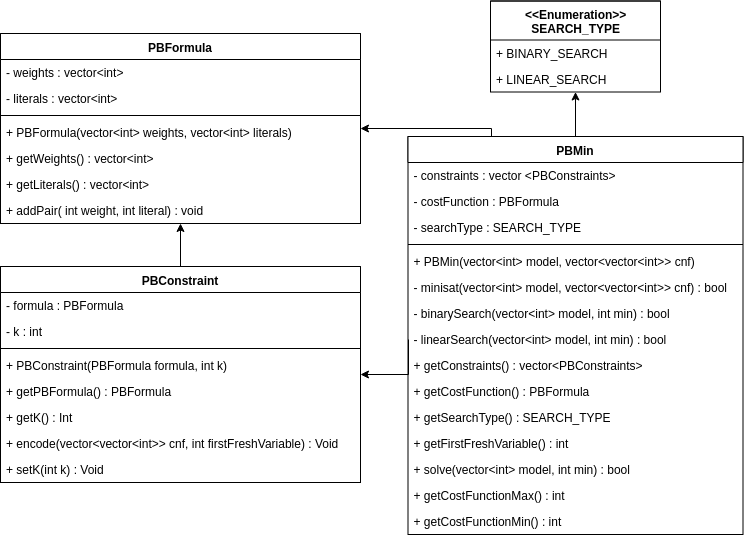
\includegraphics[width=1\textwidth]{Figures/Iteration_1_Architecture.png}
	\captionof{figure}{Iteration 1 architecture}
	\label{it1arch}
\end{center}


\paragraph{PBFormula}

This class is the one responsible for representing a Pseudo-Boolean Formula. In order to make it more interoperable with PBLib, it adopted the same representation for variables and weights which are int32\_t and int64\_t respectively.  

%TODO: it is possible to talk in more detail about it) 



\paragraph{PBConstraint} 

A Pseudo-Boolean Constraint is represented as a PBFormula and a boundary.  \\
The function \emph{encode()} is responsible for converting the Pseudo-Boolean Constraints into a CNF. This encoding is the part done with PBLib. \\
Note that there is no way of specifying the relational operator of the constraint because it will always be $\leq$.  Other constraints can be easily converted into this type as specified in \cite{Abio}.

%TODO: it is possible to talk in more detail about it) 



\paragraph{PBMin} 

This class is responsible for representing a Pseudo-Boolean Minimization problem.  It is formed by a vector of PBConstraint, the cost function which is a PBFormula and the search type which is defined by the enum \emph{SEARCH\_TYPE}.  \\
This enum has two values, \emph{BINARY\_SEARCH} and \emph{LINEAR\_SEARCH}, which are the search strategies specified in the objectives of the project.  \\\\
This class has the following methods: 
\begin{itemize}
	\item \emph{minisat()} is responsible for calling the solver, Minisat, and get the model back if it exists.
	\item \emph{binarySearch()} is responsible for executing the Binary Search algorithm to find the optimal value for the problem.
	\item \emph{linearSearch()} is responsible for executing the Linear Search algorithm to find the optimal value for the problem.
	\item \emph{getFirstFreshVarialbe()} returns a value called first fresh variable which is required by PBLib in order to encode the constraints into a CNF.
	\item \emph{solve()} is called by the user once he/she wants to solve the problem.
	\item \emph{getCostFunctionMax()} returns the maximum possible value for the cost function.
	\item \emph{getCostFunctionMin()} returns the minimum possible value for the cost function.
\end{itemize}
As the reader may have noticed, this contradicts the initial intention which was that this class should be only responsible for representing a Pseudo-Boolean Minimization problem. The methods listed above show that the class is also responsible for calling Minisat, implementing the search strategies and, as a consequence of this, calling PBLib for encoding the problem into a CNF.  

\begin{verse}
	This error in the class design had a negative impact on the next iteration which required a redesign of the architecture. It will be explained in \ref{arch-error}.
\end{verse}

\subsection{Development and TDD}

The developed started with the leaf class at the hierarchy, as seen in the architecture\ref{it1arch}, PBFormula.  \\
%TODO: Explain in more detail the development) 
Following the hierarchy, the next one was PBConstraint and the last one PBMin. \\\\
The first implemented method from PBMin was \emph{int32\_t PBMin::getFirstFreshVariable()}. This method has to return the next available literal to be used in the future by PBLib. To achieve this behaviour, this method looks at all the literals that are in the PBMin (constraints and cost function) and returns the maximum absolute literal found plus one.  \\
For example, if we have the constraint $3*1 + 2*(-2) \leq 3$, and the cost function $4*(-1) + 7*2$, the first fresh variable is 3. \\\\
The methods \emph{int64\_t PBMin::getCostFunctionMax()} and \emph{int64\_t PBMin::getCostFunctionMin()} are required to limit the search strategies. The optimal value has to be comprehended between these limits.  \\
The first part of these two methods does the same: For each literal at the cost function sums the weights where it appears positive and the weights where it appears negated and stores them in \emph{positive[i]} and \emph{negative[i]} where $i$ is the literal.\\
The maximum value for the cost function is that where a literal is set to true if \emph{positive[i]} is bigger than \emph{negative[i]}. Similarly, the minimum value for the cost function is that where a literal is set to true if \emph{negative[i]} is bigger than \emph{positive[i]}.\\\\
For example, given the cost function $-1*1 - 3*(-1) + 7*2 -5*(-2)$,\\
\emph{positive = \{-1,7\}}\\
\emph{negative = \{-3,-5\}}\\
Literal $1$ is set to $true$ because $positive[1] > negative[1]$.\\
Literal $2$ is set to $true$ because $positive[2] > negative[2]$.\\
The maximum value for the cost function is $6$.\\
Literal $1$ is set to $false$ because $positive[1] > negative[1]$.\\
Literal $2$ is set to $false$ because $positive[2] > negative[2]$.\\
The minimum value for the cost function is $-8$.\\\\
bool PBMin::binarySearch(std::vector< int32\_t > \& model, int64\_t \& min) \\
bool PBMin::linearSearch(std::vector< int32\_t > \& model, int64\_t \& min) 

\subsection{Finalization}

At this substage, some techniques learned at the Erasmus course, Software Testing, such as Category Partition Testing were applied.  \\
%TODO: At this point, Category Partition Testing should already be explained) 
These new tests revealed some bugs in the search strategies implementation for particular values for the algorithms. 

\begin{table}[h!]
	\centering
	\begin{tabular}{|l|c|c|c|}
		\hline
		\multicolumn{1}{|c|}{Class} & \emph{min} is the first value & \emph{min} is the last value & Unsatisfiable \\ \hline
		Linear Search & \begin{tabular}[c]{@{}c@{}} $\overline{x_1} \leq 0$ \\ $x_1$ \end{tabular} & \begin{tabular}[c]{@{}c@{}} $x_1 \leq 0$ \\ $x_1$\end{tabular}  & \begin{tabular}[c]{@{}c@{}} $2x_1 \leq 1$ \\ $2\overline{x_1} \leq 1$ \\ $x_1$\end{tabular} \\ \hline
		Binary Search & \begin{tabular}[c]{@{}l@{}} $\overline{x_1} \leq 0$ \\ $5x_1 + 5x_2$\end{tabular} & \begin{tabular}[c]{@{}c@{}} $\overline{x_1} \leq 0$ \\ $3x_1 + 7x_2$ \end{tabular} & \begin{tabular}[c]{@{}c@{}} $2x_1 \leq 1$ \\ $2\overline{x_1} \leq 1$ \\ $x1$\end{tabular} \\ \hline
	\end{tabular}
	\caption{Category partition testing for \emph{Linear search} and \emph{Binary search}}
	\label{cpt}
\end{table}

\section{Objective 2: Timeout}

\subsection{Problem}
It has been previously explained that SAT is an NP-Complete problem which means that there is no known algorithm which can solve it in polynomial time. In other words it can take a lot of time to solve this type of problems. \\
For example, a CNF of 300 variables and 1200 clauses takes 50 seconds to be solved.  \\\\
Some users need a result before certain time. For instance, a delivery company need a plan every morning before 08:00 AM for their trucks,packages and drivers. Therefore some users need a result before a certain time even if it is not the optimal one.  \\\\
In order that the software was able to work with this new feature, it needed a new parameter from the user and timeout strategies.

\subsection{Possible solutions}
Two different timeout strategies were considered:  

\begin{itemize}
	\item A maximum number of seconds for each call to the solver.
	\item A maximum number of seconds for the whole problem. 
\end{itemize}
Both options were considered useful, and hence they become a goal for the development substage.   

\subsection{Planning}
Some research was done about timeout strategies for solvers.  \\
%TODO: Explain sat solvers resets) 
In order to implement the asynchronous behaviour two different approaches were considered:  

\paragraph{Threads}

Threads within the same process can communicate using shared memory. \\
Threads share the same memory space which could be a source of problems if not handled carefully. In this particular case, this is helpful because the thread would execute the solver call while the parent is waiting for the timeout.  

\paragraph{Processes}

Child processes are easier to work with but, in general, they are more expensive. This is because processes have their own code, memory space, files, registers and stack which implies that every time a new child process is created, some of the listed elements need to be copied.  \\\\\\\\
Finally, Threads was the chosen option because of the following reasons: 

\begin{itemize}
	\item They sharer memory within a process which makes communication much more manageable. In this particular project, this allowed the code to be more simple. 
	\item They are less expensive to create because no copy of memory is effectuated.
\end{itemize}
The timeout was thought to be implemented as a signal sent from the parent thread to the child thread.  


\paragraph{What happens when there is a timeout?\\}
The answer depends on the timeout strategy selected for the problem: \emph{GeneralTimeoutSolver} or \emph{SimpleTimeoutSolver}. \\\\
In the first case, the flag \emph{timeoutOccurred} is set to \emph{true}, and the last found solution is returned. With the flag, the user can know if the timeout occurred and therefore know the solution may not be optimal.  \\
In the second case, the flag \emph{timeoutOccurred} is also set to \emph{true} and the current solver execution is killed. However, the search algorithm will keep running with the next values.  
\begin{center}
	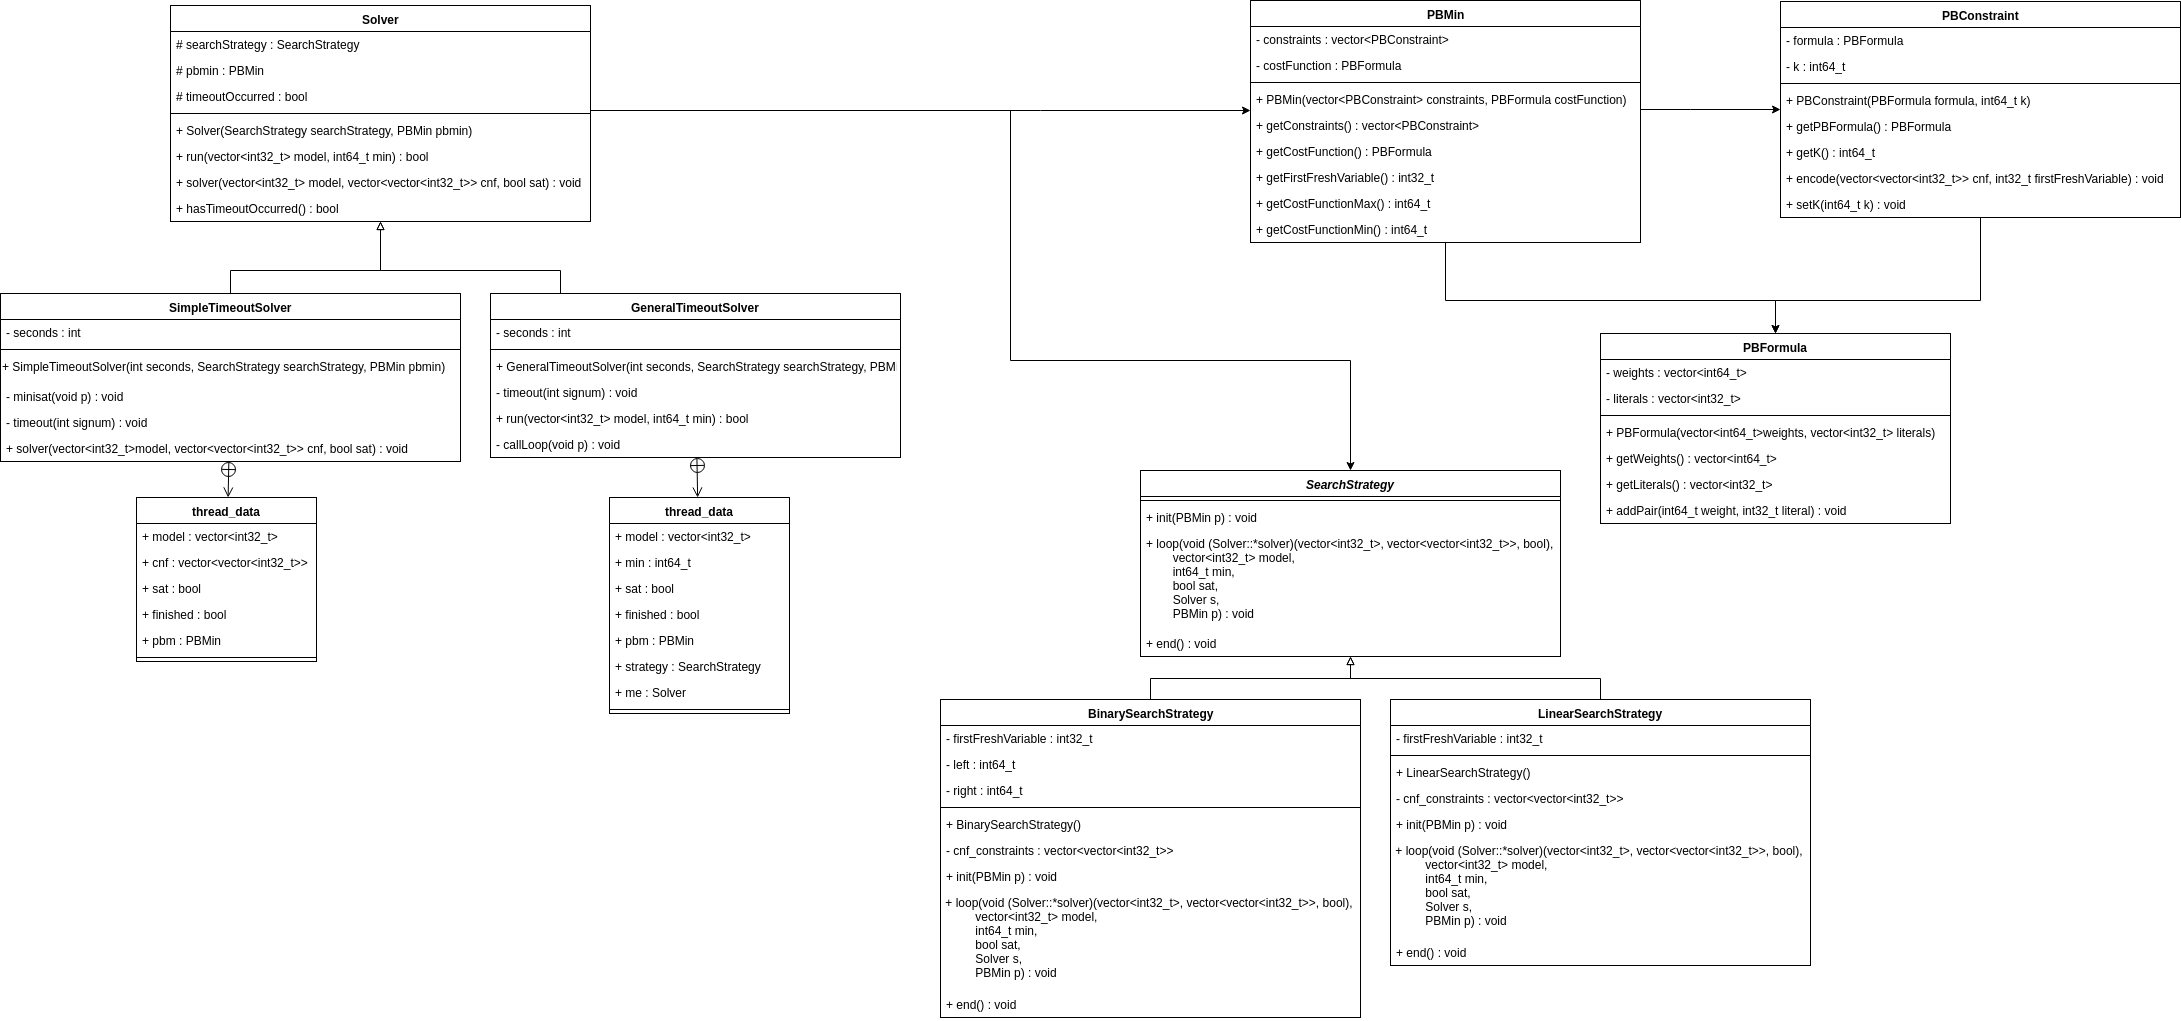
\includegraphics[width=1.6\textwidth, angle=90]{Figures/Iteration_2_Architecture-UML.png}
	\captionof{figure}{Iteration 2 architecture}
	\label{it2arch}
\end{center}
\label{arch-error}
As can be seen, the architecture suffered an evolution from the previous iteration. As previously mentioned in Iteration 1, the class PBMin was not respecting the Single responsibility principle because apart from representing the problem, it also was responsible for implementing the search strategies, calling PBLib encodings, \ldots \\ 
That architecture would have resulted in a much complex PBMin class because it would have to be responsible for the timeouts.  \\\\
For these reasons the following classes were modified or added: 
\begin{itemize}
	\item PBMin : After the refactor, this class is only responsible for representing a Pseudo-boolean minimization problem which was its original mission.
	\item SearchStrategy : One of the functionalities moved outside the PBMin class was the search strategy selection and implementation which needed to be moved to another class. For that reason, a new hierarchy of classes was created: SearchStrategy, BinarySearchStrategy and LinearSearchStrategy.  These set of classes have three methods: 
	\begin{itemize}
		\item \emph{init()}'s purpose is to prepare the class for the execution of the search algorithm. For example, encode the PBConstraints   into a CNF. 
		\item \emph{loop()}'s purpose is to execute the search algorithm.  
		\item \emph{end()} is executed after the loop once the optimal solution is found, there is no solution or a timeout occurred. It has no use by default.  
	\end{itemize}
	\item \emph{BinarySearchStrategy} uses the \emph{loop()} method to implement the binary search algorithm. 
	\item \emph{LinearSearchStrategy} uses the \emph{loop()} method to implement the linear search algorithm. 
	\item \emph{Solver} : Another behaviour removed from the PBMin class is the actual execution of the problem solver. This behaviour was moved to a new class, Solver, which is responsible for calling the SAT solver. This class is the solver without a timeout, that it is implemented by its children SimpleTimeoutSolver and GeneralTimeoutSolver. The main methods are: 
	\begin{itemize}
		\item \emph{run()} is the function called by the user once he/she wants to solve the problem.
		\item \emph{solve()} is responsible for calling the SAT solver, passing the CNF and getting back the result. 
	\end{itemize}
	\item \emph{SimpleTimeoutSolver} overrides the method \emph{solve()} and adds the creation of a thread which calls the solver while it counts for the timeout.  
	\item \emph{GeneralTimeoutSolver} overrides the method \emph{run()} and adds the creation of a thread which calls the selected search algorithm while it counts for the timeout. 
\end{itemize}  

\subsection{Development and TDD}
The first thing to do was refactor the class PBMin and move all the functionalities previously mentioned to the new classes. This also implied a refactor to the PBMin tests. Like the previous iteration, the development was done selecting classes in a bottom-up way.  \\\\
The first class created was Solver which does not implement a timeout strategy. Therefore it has the same functionality as the old PBMin: call the search algorithm and the SAT solver. As seen in the architecture diagram \ref{it2arch} this class has a dependency in the \emph{SearchStrategy} class which was not implemented at that time. To apply TDD methodology, it was necessary to create a stub. As a stub, the only purpose of \emph{SearchStrategy\_Stub} was to implement a fake behaviour in order to test the Solver class. \\
The next implemented classes were \emph{SearchStrategy}, \emph{BinarySearchStrategy} and \emph{LinearSearchStrategy} hierarchy.  \\\\
\emph{SearchStrategy} is an abstract class which means it cannot be instantiated. Its purpose is to be a "contract" between search strategies, such as linear search and binary search, and classes which use them. Because it has no code, it is not necessary to be tested.  \\
However, for its children it is mandatory. The first child, \emph{LinearSearch} implements the linear search algorithm which was in the old PBMin class. The method \emph{init()} encodes the PBConstraints of the problem into a CNF. This encoding is done at the \emph{init()} method because it has to be done only once.  \\
The method \emph{loop()} is the one which implements the algorithm. It starts defining the boundaries of the search with the maximum possible value for the cost function and its minimum.  \\
Because of the values given by the algorithm only differ in one unit, starting on the maximum and ending on the minimum, the functionality "Incremental constraints" from PBLib could be used.\\ %TODO: Explain incremental constraints PBLib)  
Finally, the method \emph{end()} does nothing. \\
The other child, \emph{BinarySearchSolver}, implements the binary search algorithm. As before, the method \emph{init()} encodes the problem constraints into a CNF. The \emph{loop()} method implements the binary search algorithm taking as the left value the minimum possible value of the cost function and as the right value its maximum. Unlike before, the incremental constraints functionality could not be used because the search is not "constant".  Finally, as before, the method \emph{end()} does nothing.  \\\\
Finally, the last classes to be implemented were \emph{SimpleTimeoutSolver} and \emph{GeneralTimeoutSolver}. \\
The Template pattern \cite{Gamma} could be applied because the children of \emph{Solver} are a specialization of it. In other words, all the hierarchy shares a lot of behaviour.  \\
The \emph{SimpleTimeoutSolver} only redefines the method \emph{solve()} to a creation of a thread which calls the sat solver with all its implications. \\
The \emph{GeneralTimeoutSolver} only redefines the method \emph{run()} to a creation of a thread which calls the function \emph{loop()} from the \emph{SearchStrategy} class.  

\subsection{Finalization}
The classes \emph{Solver}, \emph{SimpleTimeoutSolver} and \emph{GeneralTimeoutSolver}, apart from their unit tests required by TDD, were tested with integration tests.  \\
%\begin{table}[h!]
%	\centering
%	\begin{tabular}{l|l|l|l|}
%		\cline{2-4}
%		\multicolumn{1}{c|}{} & \multicolumn{1}{c|}{BinarySearchStrategy} & \multicolumn{1}{c|}{LinearSearchStrategy} & SlowSearchStrategy \\ \hline
%		\multicolumn{1}{|l|}{Solver} & Solver\_BinarySearchStrategy\_INT & Solver\_LinearSearchStrategy\_INT &  \\ \hline
%		\multicolumn{1}{|l|}{SimpleTimeoutSolver} & \begin{tabular}[c]{@{}c@{}} SimpleTimeoutSolver\_\\ BinarySearchStrategy\_INT \end{tabular} & \begin{tabular}[c]{@{}c@{}} SimpleTimeoutSolver\_ \\ LinearSearchStrategy\_INT \end{tabular}  &  \\ \hline
%		\multicolumn{1}{|l|}{GeneralTimeoutSolver} & \begin{tabular}[c]{@{}c@{}} GeneralTimeoutSolver\_ \\ BinarySearchStrategy\_INT  \end{tabular}  & \begin{tabular}[c]{@{}c@{}} GeneralTimeoutSolver\_ \\ LinearSearchStrategy\_INT \end{tabular}  & GeneralTimeoutSolver\_SlowSearchStrategy\_INT \\ \hline
%	\end{tabular}
%	\caption{Integration tests combination}
%	\label{integration-tests-combination}
%\end{table}
Integration testing was done to expose defects in the communication of classes and also test the \emph{Solver} hierarchy with real implementations of \emph{SearchStrategy} and see that the timeout was working as expected. 

% Chapter Template

\chapter{Search Algorithms} % Main chapter title

\label{Chapter4} % Change X to a consecutive number; for referencing this chapter elsewhere, use \ref{ChapterX}

In this chapter, the search algorithms used for this project are explained in more detail and how they have been adapted for this particular application.\\\\
These two search algorithms are used to find a target value in a sorted list of values. For this project, what we are trying to find is the minimum value for the cost function, and the list of values are all the integers between the minimum and the maximum possible values for the cost function.

\begin{center}
	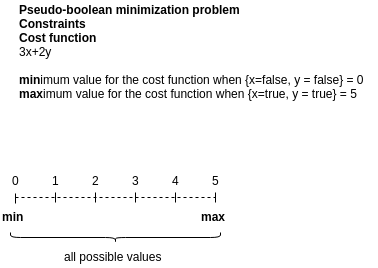
\includegraphics[width=0.8\textwidth]{Figures/Search_space.png}
	\captionof{figure}{Search Space}
	\label{search_space}
\end{center}
As the reader can see from the figure above, the search problem we are facing can be described as one where the search space is formed by integers between \emph{min} and \emph{max} and our target value is unknown.

\paragraph{How can we know that a value is the minimum, i.e. our target?\\}
If $m$ is the minimum value, we know that the constraint formed by $cost function \leq m$ is satisfiable whereas the constraint $cost function \leq m-1$ is unsatisfiable.\\
\begin{center}
	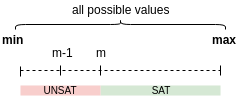
\includegraphics[width=0.8\textwidth]{Figures/SearchSpace2.png}
	\captionof{figure}{Satisfiability of the search space given a minimum value}
	\label{search_space_2}
\end{center}
This is the property used to check if the value found is minimum or not.

\section{Linear search}

Linear search is an algorithm which sequentially checks all the values for the target value until it is found or all the elements have been visited.\\
The search can start with the smallest value or the biggest one. For this application, the initial value is \emph{max} and the algorithm traverse the search space descending until \emph{min}.\\
This decision was made because proving satisfiability of a problem is easier (faster) than proving it is unsatisfiable. Also, given $m$ and $n$ where $n < m$, if $cost function \leq m$ is unsatisfiable then $cost function \leq n$ will also be unsatisfiable. \\
As previously said, the algorithm starts with \emph{max}, which means that it generates the Pseudo-Boolean constraint $cost function \leq max$. If the problem is unsatisfiable with this value, it can be deduced that with other values will also be unsatisfiable and therefore the search can end.\\
Otherwise, it keeps this value as the possible minimum and tries the next one until it finds an unsatisfiable one or the \emph{min}, which is the last value to be checked.\\
Once the algorithm finished, the last found possible value becomes the minimum, or if no possible minimum was found, the problem is unsatisfiable.\\\\
The class \emph{LinearSearchStrategy}\footnote{\href{https://github.com/marcbenedi/SAT-tfg/blob/master/source_files/LinearSearchStrategy.cpp}{Source code in Github}} implements this algorithm. Let's explain its essential parts:\\\\
Firstly, the following variables are initialised:
\begin{verbatim}
int64_t min_costFunc = pm.getCostFunctionMin();
int64_t k = pm.getCostFunctionMax();
min = pm.getCostFunctionMax()+1;
\end{verbatim}
\begin{itemize}
	\item \emph{min\_costFunc} is used to limit the last value to look at
	\item \emph{k} is the value it checks. As previously said, initially is the maximum possible value for the cost function
	\item \emph{min} is the last minimum value found. Initialised with an invalid value which is the maximum plus one
\end{itemize}
Then the first constraint is created. The algorithm takes advantage of the \emph{Incremental Constraints} functionality of PBLib.
\begin{verbatim}
IncPBConstraint inc_costFunction = IncPBConstraint(w_costFunction, PBLib::LEQ, k);
pb2cnf.encodeIncInital(inc_costFunction, cdb, auxVarManager);
\end{verbatim}
It creates an incremental constraint with the $cost function \leq k$ and then encodes it into a CNF.\\\\
The next part is the loop, the linear search implementation:
\begin{verbatim}
bool end = false;
while (!end) {
    if (k == min_costFunc) {
        end = true;
    }
	
    inc_costFunction.encodeNewLeq(k, cdb, auxVarManager);
	
    bool t_sat;
    (solver->*solve)(temp_model, cdb.getClauses(),t_sat);
	
    if (t_sat) {
        model = temp_model;
        min = k;
        k--;
    }
    else{
        end = true;
    }
}
\end{verbatim}
The loop can end for two reasons:
\begin{itemize}
	\item \emph{k == min\_costFunc}: this is the last value to check
	\item \emph{t\_sat is false}: the current iteration is unsatisfiable, i.e. the next values in the search space will also be unsatisfiable 
\end{itemize}
After encoding the new constraint $cost function \leq k$, it calls the solver.\\\\
If it is \emph{satisfiable}, the model is stored and $k$ is stored as the las $min$ found.\\
If after ending the search no other minimum has been found, that is returned along with its model. After that, a new iteration is done with $k=k-1$.

\section{Binary search}
Binary search is an algorithm which looks for a value in a given sorted input.\\
As before, our inputs is the integers between \emph{min} and \emph{max}, and therefore they are sorted.\\
In the beginning, Binary search takes the middle value and compares it with the target value. If it is bigger than the target, then it looks for the value in the subspace between minimum value and the value before the middle one. If it is smaller than the target, then it looks for the value in the subspace between the value after the middle one and the maximum.\\
For this application, the leftmost value of the search is \emph{min}, and the rightmost value for the search is \emph{max}. Again, our target value is the minimum one. For each iteration, the algorithm checks that the left side of the problem is less or equal than the right side because otherwise, the state of the search would be incorrect. \\
If this is true, then it gets the middle value between them and generates the constraint $cost function \leq middle value$, which is added with the other constraints and then encoded into a CNF. If the CNF is satisfiable, then the middle value is stored as a possible minimum, and the search continues with a new space contained between the left side and the integer between the middle value. Otherwise, if the CNF is unsatisfiable, it checks if the stored possible minimum is exactly the integer after the middle value because then the integer would be the minimum value.\\
If not, it continues the search with a new space contained between the integer after the middle value and the right side.\\\\
The class \emph{BinarySearchStrategy}\footnote{\href{https://github.com/marcbenedi/SAT-tfg/blob/master/source_files/BinarySearchStrategy.cpp}{Source code in Github}} implements this algorithm:\\\\
As previously said, the search space is limited between \emph{min} and \emph{max}. For this reason, the variables \emph{left} and \emph{right} are initialised as following:
\begin{verbatim}
left = p.getCostFunctionMin();
right = p.getCostFunctionMax();
\end{verbatim}
As in \emph{LinearSearchStrategy}, the value \emph{min} is initialised as the maximum value for the cost function plus one.
\begin{verbatim}
min = right + 1;
\end{verbatim}
Let's now explain the loop which implements the binary search algorithm:
\begin{verbatim}
while (not end) {
    if(left<=right){
        cnf.clear();
        cnf.insert(cnf.end(),cnf_constraints.begin(),cnf_constraints.end());
    
        int64_t k = (left+right)/2;
    
        if (left == right) {
            //no more values to try
            end = true;
        }
    
        firstFreshVariable = pb2cnf.encodeLeq(pm.getCostFunction().getWeights(), pm.getCostFunction().getLiterals(), k, cnf, firstFreshVariable) + 1;
    
        bool t_sat;
        (solver->*solve)(temp_model, cnf,t_sat);
    
        if (t_sat) {
            min = k;
            right = k-1;
            model = temp_model;
        }
        else{
            if (min == k + 1) {
                end = true;
            }
            left = k+1;
        }
    }
    else{
        end = true;
    }
}
\end{verbatim}
The search can end for three reasons:
\begin{itemize}
	\item \emph{left==right}: it is checking the last value, therefore there are no values left for the next iterations
	\item \emph{k unsatisfiable but k+1 satisfiable}: then \emph{k+1} is the minimum and the search finishes
	\item \emph{left > right}: the state of the search is inconsistent because it has checked all the values of the space
\end{itemize}
The first thing it does is clean the CNF and inserting the constraints of the problem again. Then, it calculates the next value to check, which is the one in the middle, and generates the constraint $cost function \leq k$. Finally, the CNF is passed to the solver.\\\\
If the CNF is \emph{satisfiable}, then \emph{k} is stored as the las minimum seen along with its model. The right side of the space is limited to \emph{k-1}.\\
Otherwise, the left side of the space is limited to \emph{k+1}, and as previously said, it checks if the last minimum value found equals \emph{k+1}.
% Chapter Template

\chapter{Timeouts} % Main chapter title

\label{Chapter5} % Change X to a consecutive number; for referencing this chapter elsewhere, use \ref{ChapterX}

In this chapter, the two timeout strategies developed for this project are explained.\\\\
As previously said in this document, some users may need a result before a specific time. When timeouts are used, the solution to the problem may not be the optimal one, as explained in the following lines.

\section{Simple timeout}
For this strategy, the user defines a maximum number of seconds that each call to the sat-solver can take. In other words, the amount of time that a value between \emph{min} and \emph{max} is checked to be the optimal or not. \\\\
To accomplish this behaviour, a new thread is created, and the call to the sat-solver is executed in parallel while the main thread looks that the elapsed time is less than the timeout defined by the user.  \\\\
When the elapsed time is longer than the time defined by the user, the main thread kills the sat-solver execution and assumes that the problem was \emph{unsatisfiable}. This assumption leads to suboptimal solutions but correct solutions. However, if the assumption were that the problem was \emph{satisfiable}, then this could point to wrong solutions. \\\\
For example:
\subsection{Linear search}
\begin{center}
	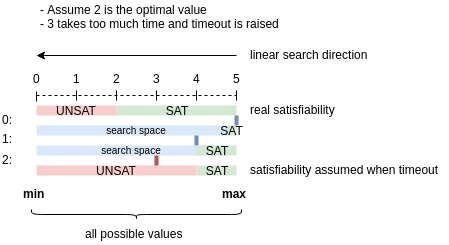
\includegraphics[width=0.8\textwidth]{Figures/SimpleTimeoutLinearSearch.png}
	\captionof{figure}{Simple timeout with linear search}
	\label{SimpleTimeoutLinearSearch}
\end{center}
As the reader can see in the figure above [\ref{SimpleTimeoutLinearSearch}], there is a Pseudo-Boolean minimisation problem which its minimum value is 2, and the cost function values go from 0 to 5. Because it is using \emph{Linear search} algorithm, it will start from 5 and will descend until the problem is \emph{unsatisfiable} or 0.\\
If 2 is the minimum value, it means that below 2 all is \emph{unsatisfiable} and from all values greater equal than 2 are \emph{satisfiable}. We also assume that the call to the sat-solver when trying 3 will take longer than the time defined by the user, i.e. a timeout will be raised. \\\\
At the first iteration of the algorithm, \emph{0:}, the CNF Pseudo-Boolean constraints AND $cost \ function \leq 5$ will be generated which will return SAT.\\
At the second iteration, \emph{1:}, the CNF Pseudo-Boolean constraints AND $cost \ function \leq 4$ will be generated, and this also will return SAT.\\
At the third iteration, \emph{2:}, the CNF Pseudo-Boolean constraints AND $cost \ function \leq 3$ will be generated. We know that this should return satisfiable but because it takes too long, the timeout is raised, and unsatisfiable is returned. The algorithm assumes that all the values below 3 will also be unsatisfiable and ends the search. 4 was the last satisfiable value found, so it is returned as the minimum value. \\\\
As the reader can see, this is not the optimal solution but a correct one.

\subsection{Binary search}
\begin{center}
	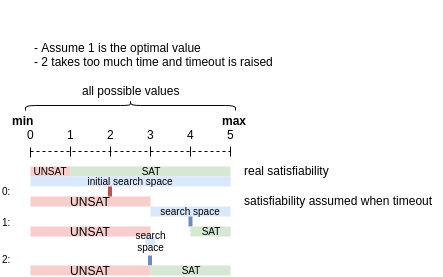
\includegraphics[width=0.8\textwidth]{Figures/SimpleTimeoutBinarySearch.png}
	\captionof{figure}{Simple timeout with binary search}
	\label{SimpleTimeoutBinarySearch}
\end{center}
In this case, the search algorithm used is \emph{Binary search}. We assume a Pseudo-Boolean minimisation problem where the minimum value is 1, the values of the cost function are between 0 ad 5, and that the call to the sat-solver when trying 2 will take longer than the time defined by the user, i.e. a timeout will be raised.\\\\
At the first iteration, \emph{0:}, the search space is between 0 and 5, and the algorithm knows nothing about the satisfiability of the problem. 2 is the middle value so the CNF Pseudo-Boolean constraints AND $cost \ function \leq 2$ is generated. Because of the problem definition, this is satisfiable, but it takes longer than the time defined by the user and the timeout is raised.\\
The execution of the sat-solver is stopped, and it assumes the CNF is unsatisfiable.\\\\
At this point, it assumes that 2 and all the values under it are unsatisfiable and the search space is reduced to 3 to 5.\\
Iterations \emph{1:}, \emph{2:} proceed as a regular Binary search execution, and finally, the value 3 is returned as the optimal one.\\\\
As before, the given solution is not optimal but correct.

\section{General timeout}
For this strategy, the user defines a maximum number of seconds that the whole problem can take. In other words, the amount of time that the user will wait for an answer. \\\\
To accomplish this behaviour, a new thread is created, and the call to the search algorithm is executed in parallel while the main thread looks that the elapsed time is less than the timeout defined by the user.  \\\\
When the elapsed time is longer than the time defined by the user, the main thread kills the search algorithm execution and assumes that it finished normally, i.e. the last value found is returned as the minimum one. %This assumption leads to suboptimal solutions but correct solutions. However, if the assumption were that the problem was satisfiable, then this could point to wrong solutions. 
\subsection{Linear search}
\begin{center}
	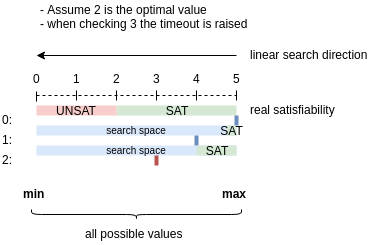
\includegraphics[width=0.8\textwidth]{Figures/GeneralTimeoutLinearSearch.png}
	\captionof{figure}{General timeout with linear search}
	\label{GeneralTimeoutLinearSearch}
\end{center}
As the reader can see in the figure above [\ref{GeneralTimeoutLinearSearch}], there is a Pseudo-Boolean minimisation problem which its minimum value is 2, and the cost function values go from 0 to 5. Because it is using Linear search algorithm, it will start from 5 and will descend until the problem is unsatisfiable or 0. \\
If 2 is the minimum value, it means that below 2 all is unsatisfiable and from all values greater equal than 2 are satisfiable.  We also assume that trying 3 will take longer than the time defined by the user, i.e. a timeout will be raised.\\\\
At the first iteration of the algorithm, \emph{0:}, the CNF Pseudo-Boolean constraints AND $cost \ function \leq 5$ will be generated which will return SAT.\\
At the second iteration, \emph{1:}, the CNF Pseudo-Boolean constraints AND $cost \ function \leq 4$ will be generated, and this also will return SAT.\\
At the third iteration, \emph{2:}, the CNF Pseudo-Boolean constraints AND $cost \ function \leq 3$ will be generated. Then the timeout is raised, and the last satisfiable value found, 4, is returned as the minimum one.\\\\
As the reader can see, this is not the optimal solution but a correct one. 

\subsection{Binary search}
\begin{center}
	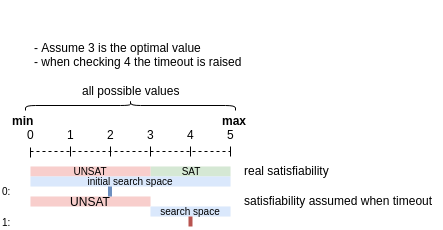
\includegraphics[width=0.8\textwidth]{Figures/GeneralTimeoutBinarySearch.png}
	\captionof{figure}{General timeout with binary search}
	\label{GeneralTimeoutBinarySearch}
\end{center}
In this case, the search algorithm used is Binary search. We assume a Pseudo-Boolean minimisation problem where the minimum value is 3, the values of the cost function are between 0 and 5, and that when trying 4 the timeout will be raised. \\\\
At the first iteration, \emph{0:}, the search space is between 0 and 5, and the algorithm knows nothing about the satisfiability of the problem. 2 is the middle value so the CNF Pseudo-Boolean constraints AND $cost \ function \leq 2$ is generated. Because 2 is unsatisfiable, the search space is reduced to 3 to 5, and the next value to be checked is 4. \\\\
When checking 4, the timeout is raised, and the search space becomes empty. Because there are no more elements to be checked, the last minimum value found is returned, which in this case there is no one, i.e. the software returns unsatisfiable. 
\chapter{Project Planning}
\label{Chapter4}

\section{Schedule}
\subsection{Estimated project duration}
For this project there have been estimated 450 hours of work, starting on \textbf{19th of February} and ending on \textbf{23rd of June}.\\

\subsection{Considerations}
The original plan could be modified to be adapted to deviations. Agile methodology implies that some new requirements can appear which could modify the planning. It is hard to do a realistic planning with Agile methodology because the iteration's requirements are not fully known until the Planning stage.\\\\
Because this project will be developed sequentially by only one person, the creation of a PERT diagram has been discarded. Nevertheless, some part of the documentation will be done in parallel.

\section{Resources}
For the development of this project, three types of resources will be needed.
\subsection{Human Resources}
\begin{itemize}
	\item One person working 20 hours per week until the finalization of the project.
\end{itemize}
\subsection{Material Resources}
\begin{itemize}
	\item Lenovo IdeaPad U330T\\
	This laptop will be used to write the documentation and develop the project.
\end{itemize}
\subsection{Software Resources}
\begin{itemize}
	\item Trello: Web application to manage project tasks.
	\item teXstudio: LateX editor to write all the documentation.
	\item e-mail: Communication tool used to contact the supervisor. 
	\item Atom: Text editor to write the code.
	\item Git: VCS to backup and keep tracking of the project.
	\item C++: Language used for the development.
	\item PBLib: C++ library for Pseudo-Boolean encodings.
	\item CLion: Code editor focused on C++.
	\item Google Test: Unit testing framework for C++ developed by Google.
\end{itemize}

\section{Project Planning}

\subsubsection{GEP}
This task corresponds to the work done during the GEP course. This task has not any dependency but the work done will be used for the final documentation.\\

The estimated time for this stage is 70 hours.
\subsubsection{Requirements analysis, architecture and debugging}
This stage will be used for defining the requisites to accomplish, the architecture of the software and refactor the previous code. Also, the required tools will be installed. \\

The estimated time for this stage is 90 hours.
\subsubsection{Iterations}
Because Agile methodology will be followed, the project has been divided into iterations. There will be a total of 3 iterations: Pseudo-Boolean minimisation, Timeout strategies, and Multithreading being this last one optional. \\

For each iteration, 80h of work are estimated.
\paragraph{Planning\\}
This stage will be used for defining the scope of the iteration and goals.\\

This stage will be 10 hours long.
\paragraph{Development and TDD\\}
In this stage, the iteration will be developed and tested.\\

This stage will be 60 hours long.
\paragraph{Finalization\\}
In this stage, all possible bugs will be solved, and feedback from the supervisor will be taken.\\

This stage will be 10 hours long.


\subsubsection{Final Stage}
Here, all the development will be finished, and it will be used for finishing all the documentation and prepare the final presentation.\\

This stage will take 50 hours.

\subsection{Gantt Diagram}
\begin{figure}[hbtp] 
	\centering
	\makebox[\textwidth]{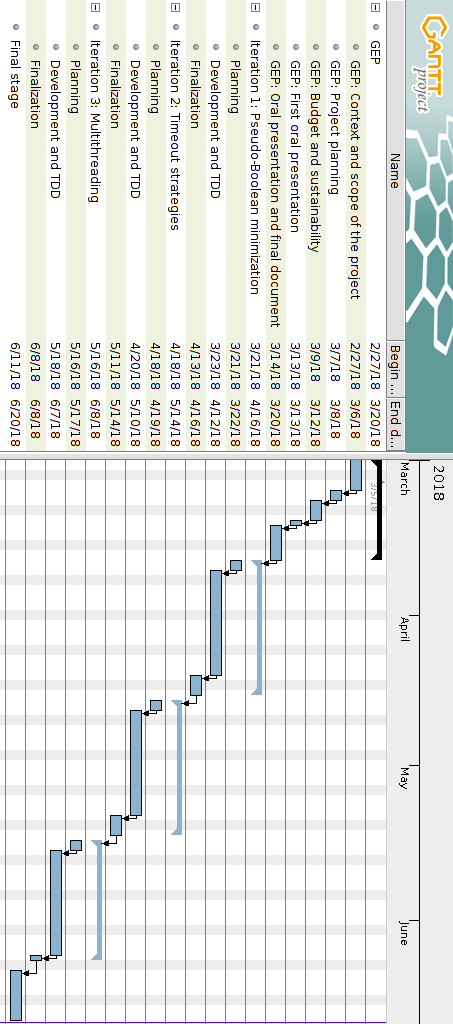
\includegraphics[height=.60\paperheight]{Figures/GanttTable2.png}}
	\caption{Gantt diagram of the project}
	\label{GanttDiagram}
\end{figure}
%todo: arreglar el diagrama. li falta la initial stage


\section{Alternatives and Action Plans}
Because of using an Agile methodology, the project functionalities can be easily adapted during the development. \\

\subsection{Potential deviations}
\subsubsection{Incorrect estimations}
It could be that the purposed estimations are not correct and be underestimated or overestimated. In the first case, if some iteration takes less time than expected, the next iteration will be started immediately. On the other case, if an iteration takes more time than expected, more hours will be added, for example, weekend hours. \\
If even with this countermeasures the iteration is delaying the project some optional improvements will be discarded in order to guarantee the main functionalities and the project would be finished before the deadline. 
The effect on the resources would be more electricity consumed by the laptop on the added hours. 

\subsubsection{Summer internship}

The deadline for this project is the 23rd of June. 
The author applied for a CERN internship from 4th of June until 31st of August. \\\
In case of being accepted into the program, the final stage would have to be done during the internship. Since the final stage is for doing the final document and the final presentation, it can be lightened by paralleling part of its work during other stages.\\
The duration of the project is not affected because the only thing that would be done is a different distribution of the work. For the same reason, it would not have any effect on the resources.

\subsubsection{Compatibility issues}

As explained before, PBLib could cause some compatibility issues with the existing software which works with another library, Cudd. \\
If this happens, in the best case some hours will be spent fixing this issue or finding a substitute. In the worst situation, the functionalities of PBLib would have to be implemented which would take much time. The project duration could be affected, but it would be always be finished before the deadline using weekend hours. The resources which will be used in addition is more electricity consumed by the laptop.

\subsubsection{Base project code quality}
The existing project could have some quality issues and be a source of bugs which would cause many delays. For these reasons, the first stage of this project will be focused on assuring quality code of the existing project.  The project duration would not be affected because part of the first stage is focused on that guaranteeing project finalization.\\\\\\
As explained in each possible deviation, the priority is finishing the project before the deadline.  As said, extra-hours from the weekend can be used to work on the project to accomplish all the objectives. If even these hours are not enough, then the optional objective \emph{Multithreading} will not be done. 

\section{Project execution}%TODO: name, maybe real plan

In this section, an analysis of the project execution is done.

% Please add the following required packages to your document preamble:
% \usepackage{graphicx}
\begin{table}[hbtp]
	\centering
	\resizebox{\textwidth}{!}{%
		\begin{tabular}{|l|r|r|}
			\hline
			\multicolumn{1}{|c|}{Stage}  & \multicolumn{1}{c|}{Expected hours} & \multicolumn{1}{c|}{Real hours} \\ \hline
			GEP & 70 & 70 \\ \hline
			Requirement analysis, architecture and debugging &   90 & 75 \\ \hline
			Iteration 1: PB Minimisation & 80 & 87 \\ \hline
			Iteration 2: Timeout  & 80 & 88 \\ \hline
			Iteration 3: Multithreading  & 80 & - \\ \hline
			Finalization & 50 & 65 \\ \hline\hline
			Total & 450 & 385 \\ \hline
		\end{tabular}%
	}
	\caption{Planned time and real time per stage}
		\label{planned-real-time}
\end{table}
The first deviation is at \emph{Requirement analysis, architecture and debugging}. The expected hours were 90 but the required were 75. This is because when applying testing methods to the code the amount of errors found was less than expected.\\\\
\emph{Iteration 1: Pseudo-Boolean minimisation} and \emph{Iteration 2: Timeout} took more time than expected specially the second one because of the refactor of the architecture.\\\\
In the original plan, after the second iteration came \emph{Iteration 3: Multi-threading}. As already said, the third iteration was optional so instead of it, the author started the final stage. The decision was made knowing that during June he would be doing a full-time internship which would reduce the available time to work on the project significantly.

\chapter{Economic Management}
\label{Chapter7}

In this section, all the costs of the project are exposed. 
\section{Direct costs}
Direct costs are those that have a direct relationship with the manufacture of the product. In this case, the only direct costs are the human resources. 

\subsection{Human resources}
The cost of the human resources has been estimated with the following expression: $Cost = \frac{Salary}{Hour} \times Expected Hours$. The salaries have been extracted from PagePersonnel study\cite{PagePersonnel}. In this study, the salaries are expressed per year. In average, there are 1.500 working hours per year. To obtain the price per hour, the salary per year has been divided by the working hours per year.\\\\
Taking into consideration the Gantt chart from the previous deliverable, the dedication of each role has been defined as follows:

\begin{table}[h!]
	\centering
	\begin{tabular}{|l|r|r|r|}
		\hline
		Stage & \multicolumn{1}{l|}{Project Manager} & \multicolumn{1}{l|}{Software Architect} & \multicolumn{1}{l|}{Developer} \\ \hline
		GEP & 70 & 0 & 0 \\ \hline
		Initial Stage & 30 & 30 & 30 \\ \hline
		Iteration 1,2,3 & 6 & 147 & 87 \\ \hline
		Final Stage & 30 & 0 & 20 \\ \hline
	\end{tabular}
	\caption{Hours destined to each stage per role}
	\label{StageResources}
\end{table}
\begin{table}[h!]
	\centering
	\begin{tabular}{|l|r|r|r|}
		\hline
		Role & \multicolumn{1}{l|}{Estimated hours (h)} & \multicolumn{1}{l|}{Price/hour (€)} & \multicolumn{1}{l|}{Total cost (€)} \\ \hline
		Project Manager & 136 & 27  & 3.672 \\ \hline
		Software Architect & 177 & 25 & 4.425 \\ \hline
		Developer & 137 & 14 & 1.918 \\ \hline\hline
		Total & \multicolumn{3}{r|}{10.015} \\ \hline
	\end{tabular}
	\caption{Human resources budget}
	\label{HumanResources}
\end{table}

\section{Indirect costs}
Indirect costs are those that do not have a direct relationship with the manufacture of the product. In this case, the indirect costs are Hardware, Software, and some others. 

\subsection{Hardware}

According to \emph{Agencia Tributaria}\footnote{\href{http://www.agenciatributaria.es/AEAT.internet/en_gb/Inicio/_Segmentos_/Empresas_y_profesionales/Empresas/Impuesto_sobre_Sociedades/Periodos_impositivos_a_partir_de_1_1_2015/Base_imponible/Amortizacion/Tabla_de_coeficientes_de_amortizacion_lineal_.shtml} {Agencia Tributaria - amortizations}}, the maximum number of years to amortize a computer equipment is 8. Therefore the amortization of Hardware resources has been calculated following this expression: $Amortization = \frac{Price}{8\times12} \times 5$

\begin{table}[h!]
	\centering
	\begin{tabular}{|l|r|r|r|r|}
		\hline
		Product & \multicolumn{1}{l|}{Price (€)} & \multicolumn{1}{l|}{Units} & \multicolumn{1}{l|}{Useful life (y)} & \multicolumn{1}{l|}{Amortization (€)} \\ \hline
		Lenovo IdeaPad U330T & 899 & 1 & 8 & 46,83\\ \hline\hline
		Total & \multicolumn{4}{r|}{46,83} \\ \hline
	\end{tabular}
	\caption{Hardware resources budget}
	\label{HardwareResources}
\end{table}

\subsection{Software}
For software resources, free tools have been selected, and student discounts have been used to minimise the total cost.
\begin{table}[h!]
	\centering
	\begin{tabular}{|l|r|r|r|r|}
		\hline
		Product              & \multicolumn{1}{l|}{Price (€)} & \multicolumn{1}{l|}{Units} & \multicolumn{1}{l|}{Useful life (y)} & \multicolumn{1}{l|}{Amortization (€)} \\ \hline
		GitHub	& 6,10/month & 5 & N/A & 30,5 \\ \hline
		GitHub student pack & -6,10/month & 5 & N/A & -30,5 \\ \hline
		Clion 	& 6,90/month & 5 & N/A & 34,5 \\ \hline
		JetBrains Product Pack for Students & -6,90/month & 5 & N/A & -34,5 \\ \hline
		Atom 	& 0,00 & 1 & N/A & 0,00 \\ \hline
		TeXstudio 	& 0,00 & 1 & N/A & 0,00 \\ \hline\hline
		Total	& \multicolumn{4}{r|}{0,00}                                                                                           \\ \hline
	\end{tabular}
	\caption{Software resources budget}
	\label{SoftwareResources}
\end{table}

\subsection{Other resources}
Internet connexion price has been extracted from Pepephone\footnote{\href{https://www.pepephone.com/internet-en-casa}{Pepephone fibra}} plan, which is 34,6€ per month. \\
kWh price has been extracted from \href{https://tarifasgasluz.com/faq/precio-kwh-espana-2017}{Selectra}. The average price per kWh is 0,12€.
In office supplies paper packs, books, pens, \ldots \ are included.
\begin{table}[h!]
	\centering
	\begin{tabular}{|l|r|r|r|}
		\hline
		\multicolumn{1}{|l|}{Product} & \multicolumn{1}{l|}{Price(€)} & \multicolumn{1}{l|}{Units} & \multicolumn{1}{l|}{Total (€)} \\ \hline
		Internet connexion & 0,047/h & 450 hours & 21,15\\ \hline
		Power consumption & 51Wh & 450 hours & 2,75 \\ \hline
		Print & 0,05/page & 400 pages & 20 \\ \hline
		Office supplies & 50 & 1 & 50 \\ \hline\hline
		Total & \multicolumn{3}{r|}{93,9}                                                                        \\ \hline
	\end{tabular}
	\caption{Other resources budget}
	\label{OtherResources}
\end{table}

\section{Contingency}
The contingency percentage for direct costs has been estimated following the author's experience on past projects. For indirect costs, the budget is more straightforward to estimate therefore a small percentage has been selected.
\begin{table}[h!]
	\centering
	\begin{tabular}{|l|r|r|r|}
		\hline
		\multicolumn{1}{|l|}{Concept} & \multicolumn{1}{l|}{Price (€)} & \multicolumn{1}{l|}{Percentage (\%)} & \multicolumn{1}{l|}{Total (€)} \\ \hline
		Direct costs & 10.015 & 30 & 3.004,5 \\ \hline
		Indirect costs & 140,73 & 15 & 21,11\\ \hline\hline
		Total & \multicolumn{3}{r|}{3.025,61} \\ \hline
	\end{tabular}
	\caption{Contingency budget}
	\label{Contingency}
\end{table}

\section{Unforeseen}
The first unforeseen is that the computer breaks. In this case, a new one will be bought. The other unforeseen events are that the stages of the project being extended. For each stage, a 50\% delay has been estimated.
\begin{table}[h!]
	\centering
	\begin{tabular}{|l|r|r|r|}
		\hline
		Unforeseen & \multicolumn{1}{l|}{Cost (€)} & \multicolumn{1}{l|}{Probability (\%)} & \multicolumn{1}{l|}{Total (€)} \\ \hline
		Broken computer & 1.300 & 5 & 65 \\ \hline
		Delay GEP stage & 945 & 15 & 141,75\\ \hline
		Delay initial stage & 990 & 15 & 148,5\\ \hline
		Delay iteration 1 & 842,5 & 15 & 126,38\\ \hline
		Delay iteration 2 & 842,5 & 15 & 126,38\\ \hline
		Delay iteration 3 & 842,5 & 15 & 126,38\\ \hline
		Delay final stage & 545 & 15 & 81,75\\ \hline\hline
		Total & \multicolumn{3}{r|}{816,14} \\ \hline
	\end{tabular}
	\caption{Unforeseen budget}
	\label{Unforeseen}
\end{table}

\section{Total budget}
In conclusion, the total budget of the project is:
\begin{table}[h!]
	\centering
	\begin{tabular}{l|r|}
		\cline{2-2}
		& \multicolumn{1}{l|}{Cost (€)} \\ \hline
		\multicolumn{1}{|l|}{Direct costs} & 10.015\\ \hline
		\multicolumn{1}{|l|}{Indirect costs}& 140,73\\ \hline
		\multicolumn{1}{|l|}{Contingency} & 3.025,61\\ \hline
		\multicolumn{1}{|l|}{Unforeseen} & 816,14\\ \hline\hline
		\multicolumn{1}{|l|}{Total} & 13.997,48\\ \hline
	\end{tabular}
	\caption{Total budget}
	\label{TotalBudget}
\end{table}
\section{Control management}
The control management mechanisms will be used to study and compare deviations.\\\\
The Human Resources is an initial estimation, therefore, the estimated cost and the real cost obtained once the project is finished will be compared. In any case, an hour follow-up will be done for each iteration and the functionalities implemented to see if the planning is accurate, or correct possible deviations and decide which functionalities could be added or deleted in order to accomplish the planning. Another method to solve the possible deviations could be reorganizing the Gantt chart. \\\\
At the end of the project, the original estimated budget will be compared with the real one. Finally, a study of which deviations and unforeseen appeared will be done and check if they can be covered by the contingency budget. This analysis will be very useful to do future budgets and to apply the extracted conclusions. \\\\
The indicators used for that are: Variance in cost by rate, efficiency variance, variance in totals, \ldots

\section{Real budget}

In this section, an analysis of the deviation on the budget is done.

\subsubsection{Direct costs}

\begin{table}[h!]
	\centering
		\begin{tabular}{|l|r|r|r|}
			\hline
			\multicolumn{1}{|c|}{Stage} & \multicolumn{1}{c|}{Product Manager} & \multicolumn{1}{c|}{Software Architect} & \multicolumn{1}{c|}{Developer} \\ \hline
			GEP & 70 & 0 & 0 \\ \hline
			\begin{tabular}[c]{@{}l@{}}Requirement analysis, \\ architecture and debuggin\end{tabular} & 30 & 30 & 15 \\ \hline
			\begin{tabular}[c]{@{}l@{}}Iteration 1: \\ Pseudo-Boolean minimisation\end{tabular} & 2 & 49 & 36 \\ \hline
			Iteration 2: Timeout & 2 & 49 & 37 \\ \hline
			Final Stage & 60 & 0 & 5 \\ \hline
		\end{tabular}%
	
	\caption{Hours per role}
	\label{hours-role}
\end{table}
In this table\ref{hours-role}, the hours of each iteration are divided per role. 

% Please add the following required packages to your document preamble:
% \usepackage{graphicx}
\begin{table}[h!]
	\centering
		\begin{tabular}{|l|r|r|r|}
			\hline
			\multicolumn{1}{|c|}{Role} & \multicolumn{1}{c|}{Price/Hour} & \multicolumn{1}{c|}{Hours} & \multicolumn{1}{c|}{Cost (€)} \\ \hline
			Product Manager & 27,00 & 164 & 4.428,00 \\ \hline
			Software Architect & 25,00 & 128 & 3.200,00 \\ \hline
			Developer & 14,00 & 93 & 1.302,00 \\ \hline\hline
			Total & \multicolumn{3}{r|}{8.930,00} \\ \hline
		\end{tabular}%
	\caption{Real cost of human resources}
	\label{real-hr}
\end{table}
As the reader can see, the direct costs have been smaller than expected. As explained in the previous chapter\ref{Chapter4}, the Iteration 3: Multi-threading has not been done therefore the number of hours for each role has also decreased. 

\subsubsection{Indirect costs}
There has been two additions to the Indirect Costs for the project which is a new software: 
\begin{itemize}
	\item Grammarly\footnote{https://www.grammarly.com}: The Grammarly Premium feature was bought in order to improve the English level for the document.
	\item Transport: In order to do the final presentation, a plant ticket from Geneva to Barcelona was required.
\end{itemize}


\begin{table}[h!]
	\centering
	\begin{tabular}{|l|r|r|r|}
		\hline
		\multicolumn{1}{|l|}{Product} & \multicolumn{1}{l|}{Price(€)} & \multicolumn{1}{l|}{Units} & \multicolumn{1}{l|}{Total (€)} \\ \hline
		Grammarly Premium & 139,95  &1& 139,95\\ \hline
		Grammarly discount & -74,95 &1 & -74,95\\ \hline
		Transport & 112 & 1 & 112\\ \hline
		Total & \multicolumn{3}{r|}{177,00}                                                                        \\ \hline
	\end{tabular}
	\caption{Other resources budget}
	\label{indirect-cost-addition}
\end{table}

\subsubsection{Contingency and unforeseen}
The budget for these two cases has not been necessary and therefore they remain unchanged.
\subsubsection{Total cost}
In conclusion, the total budget of the project is:
\begin{table}[h!]
	\centering
	\begin{tabular}{l|r|}
		\cline{2-2}
		& \multicolumn{1}{l|}{Cost (€)} \\ \hline
		\multicolumn{1}{|l|}{Direct costs} & 8.930,00 \\ \hline
		\multicolumn{1}{|l|}{Indirect costs}& 257,73\\ \hline
		\multicolumn{1}{|l|}{Contingency} & 3.025,61\\ \hline
		\multicolumn{1}{|l|}{Unforeseen} & 816,14\\ \hline\hline
		\multicolumn{1}{|l|}{Total} &  13.029,48\\ \hline
	\end{tabular}
	\caption{Total cost}
	\label{real-cost}
\end{table}
The difference between the estimated cost, 13.977,48€, and the real one, 13.029,48€, is 948,00€.\\\\
As previously mentioned, the difference is due to the reduction of hours needed for the project.\\\\
However, the final price to the costumer would be 9.187,73€ because Contingency and Unforeseen budget has not been required. 
\chapter{Sustainability and Social Commitment}
\label{Chapter8}

\section{Sustainability Matrix}
In this section, the sustainability matrix is resumed according to the numbers described here\cite{MatrixPoints}.

\begin{table}[h]
	\centering
	\begin{tabular}{l|c|c|c|}
		\cline{2-4}
		& \multicolumn{1}{l|}{PPP} & Useful life & Risks \\ \hline
		\multicolumn{1}{|l|}{Environmental} & 7 & 20& -4\\ \hline
		\multicolumn{1}{|l|}{Economical} & 7 & 15 & -10\\ \hline
		\multicolumn{1}{|l|}{Social} & 8 & 15 & 0\\ \hline
		\multicolumn{1}{|l|}{Sustainability range} & \multicolumn{3}{c|}{58} \\ \hline
	\end{tabular}
	\caption{Sustainability matrix}
	\label{SustainabilityMatrix}
\end{table}


\section{Economic dimension}

\subsection{PPP}
The estimated budget of the project can be found in table \ref{TotalBudget}. The estimated budget is 13.997,48€. This number has been estimated taking into account the working hours of each role, the hardware and software used, indirect costs, contingency, and unforeseen events.
 
\subsection{Shelf life}
Nowadays, the no optimization of Pseudo-Boolean encodings implies that the problems are bigger and harder which causes a long execution and more consumption of resources. With the optimizations that this project will study, the final execution time could be reduced therefore the power needed to solve the problem which translates into a more reduced cost.

\subsection{Risks}
As exposed previously, some risks are problems with the planning, problems with the tools used,\ldots\\
The main risk is that the optimizations proposed are not useful in a practical environment. 

\section{Environmental dimension}
\subsection{PPP}
The estimated electric usage for this project can be found in this table \ref{OtherResources}. The estimation has been done with this expression: $E=\frac{W}{h} \times T$. In this project $E=\frac{51W}{1h}\times 450h = 22,950kW$\\\\
It is hard to minimize more the impact of this project. Some strategies are turning off the computer when not using it, minimizing the amount of paper used, \ldots\\
Some resources are reused, for example, instead of writing all the functionalities, some C++ libraries will be used.
\subsection{Shelf life}
It is hard to measure the footprint of this project along with all its useful life. It will depend on the success of the project, and how many people will use it. \\\\
Currently SAT problems are executed in SAT-Solvers using some optimizations. As explained before, this problem is NP-Complete which among other things implies that there is no known algorithm which can solve it in polynomial time. In other words, solving SAT is very time and resource expensive. \\
Also, SAT is widely used in many fields. For example, computational complexity, databases, programming languages, artificial intelligence and system verification. This translates into a big electricity consumption and a huge footprint. For example, the MareNostrum\cite{MareNostrum} supercomputer spends 1,3MW/year. \\\\
This project purposes more optimizations to reduce the execution time. Even if these optimisations are small, because SAT is widely used, it could have a huge impact. It will have a positive impact because it will reduce the total $CO^2$ emissions released by the computers used to solve them.

\subsection{Risks} 
The footprint of this project could be worst than expected if the development of it is extended.

\section{Social dimension}
\subsection{PPP}
This first stage of the project, GEP, will improve my management and planning skills, my English abilities, how to document and budget projects.\\
The other stages will expand my knowledge about informatics and the opportunity to put in practice a lot of skills developed during this degree. \\
Finally, my ability to present in front of people and defend the work done during these months.

\subsection{Shelf life}
This project will improve a lot of fields because SAT-Solvers are widely used. For example, Planners, Artificial Intelligence, \ldots \ which can have an unpredictable impact in the life of people.\\\\
Currently this problem is solved using other techniques. The solution that this project purposes is an addition to them (it is not exclusive). There is a real need for this type of projects because as said previously, SAT is an NP-Complete problem therefore any improvement on this field will reduce the hardness of the problem with all the consequences this implies.
\subsection{Risks}
The only negative impact that this project can have is not being used. In this case, it will not be used and the society will remain unchanged.


\chapter{Conclusions} 
\label{Chapter9}

%todo: explicar conclusions

%a que aspirava el projecte? comentar els objectius i argumentar si shan assolit

%simplificar: si

%comentar la importancia del testing TDD i de disenyar be larquitectura



\section{Future Work}


%Afegir mes parametres de configuracio

%TODO afegir a aquest document documentacio de com utilitzar el software (potser com anex?)

%Altres estrategies de timeout mes inteligents?


%----------------------------------------------------------------------------------------
%	THESIS CONTENT - APPENDICES
%----------------------------------------------------------------------------------------

\appendix % Cue to tell LaTeX that the following "chapters" are Appendices

% Appendix A

\chapter{Frequently Asked Questions} % Main appendix title

\label{AppendixA} % For referencing this appendix elsewhere, use \ref{AppendixA}

\section{How do I change the colors of links?}

The color of links can be changed to your liking using:

{\small\verb!\hypersetup{urlcolor=red}!}, or

{\small\verb!\hypersetup{citecolor=green}!}, or

{\small\verb!\hypersetup{allcolor=blue}!}.

\noindent If you want to completely hide the links, you can use:

{\small\verb!\hypersetup{allcolors=.}!}, or even better: 

{\small\verb!\hypersetup{hidelinks}!}.

\noindent If you want to have obvious links in the PDF but not the printed text, use:

{\small\verb!\hypersetup{colorlinks=false}!}.

%% Appendix A

\chapter{Search Algorithms} % Main appendix title

\label{AppendixB} % For referencing this appendix elsewhere, use 

In this appendix, the search algorithms used for this project are explained in more detail and how they have been adapted for this particular application.\\\\
These two search algorithms are used to find a target value in a sorted list of values. For this project, what we are trying to find is the minimum value for the cost function, and the list of values are all the integers between the minimum possible value for the cost function and the maximum possible value for it.

\begin{center}
	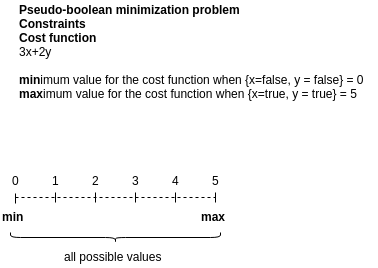
\includegraphics[width=0.8\textwidth]{Figures/Search_space.png}
	\captionof{figure}{Search Space}
	\label{search_space}
\end{center}
As the reader can see from the figure above, the search problem we are facing can be described as one where the search space is formed by integers between \emph{min} and \emph{max} and our target value is unknown.

\paragraph{How can we know that a value is the minimum, i.e. our target?\\}
If $m$ is the minimum value, we know that the constraint formed by $cost function \leq m$ is satisfiable whereas the constraint $cost function \leq m-1$ is unsatisfiable.\\\\
This is the property used to check if the value found is minimum or not.

\section{Linear search}

Linear search is an algorithm which sequentially checks all the values for the target value until it is found or all the elements have been visited.\\
The search can start with the smallest value or the biggest one. For this application, the initial value is \emph{max} and the algorithm traverse the search space descending until \emph{min}.\\
This decision was made because proving satisfiability of a problem is easier (faster) than proving it is unsatisfiable. Also, given $m$ and $n$ where $n < m$, if $cost function \leq m$ is unsatisfiable then $cost function \leq n$ will also be unsatisfiable. \\
As previously said, the algorithm starts with \emph{max}, which means that it generates the Pseudo-Boolean constraint $cost function \leq max$. If the problem is unsatisfiable with this value, it can be deduced that with other values will also be unsatisfiable and therefore the search can end.\\
Otherwise, it keeps this value as the possible minimum and tries the next one until it finds an unsatisfiable one or the \emph{min}, which is the last value to be checked.\\
Once the algorithm finished, the last found possible value becomes the minimum, or if no possible minimum was found, the problem is unsatisfiable.

\section{Binary search}
Binary search is an algorithm which looks for a value in a given sorted input.\\
As before, our inputs is the integers between \emph{min} and \emph{max}, and therefore they are sorted.\\
In the beginning, Binary search takes the middle value and compares it with the target value. If it is bigger than the target, then it looks for the value in the subspace between minimum value and the value before the middle one. If it is smaller than the target, then it looks for the value in the subspace between the value after the middle one and the maximum.\\
For this application, the leftmost value of the search is \emph{min}, and the rightmost value for the search is \emph{max}. Again, our target value is the minimum one. For each iteration, the algorithm checks that the left side of the problem is less or equal than the right side because otherwise, the state of the search would be incorrect. \\
If this is true, then it gets the middle value between them and generates the constraint $cost function \leq middle value$, which is added with the other constraints and then encoded into a CNF. If the CNF is satisfiable, then the middle value is stored as a possible minimum, and the search continues with a new space contained between the left side and the integer between the middle value. Otherwise, if the CNF is unsatisfiable, it checks if the stored possible minimum is exactly the integer after the middle value because then the integer would be the minimum value.\\
If not, it continues the search with a new space contained between the integer after the middle value and the right side.
% Appendix A

\chapter{Google Test} % Main appendix title

\label{AppendixC} % For referencing this appendix elsewhere, use 

In this appendix, Google Test is explained in more detail, along with some examples and how it has been applied to this application.

\section{Google Test}
Google Test, or Google C++ Testing Framework, is a tool developed by Google. As a Testing Framework, it allows the definition of functions called \emph{TEST()} which do two things:
\begin{itemize}
	\item Executes some functionality of the code
	\item Compares the output with the expected output to detect unexpected and erroneous behaviour.
\end{itemize}

Let us evaluate the following test:
\begin{verbatim}
TEST(FactorialTest, Positive) {
    EXPECT_EQ(1, Factorial(1));
    EXPECT_EQ(2, Factorial(2));
    EXPECT_EQ(6, Factorial(3));
    EXPECT_EQ(40320, Factorial(8));
}
\end{verbatim}
FactorialTest is the test case name which is used for defining test groups. For example, if the programmer wanted to test Factorial behaviour for negative input, he/she could have difined \emph{TEST(FactorialTest,Negative)}. Positive is the test name.\\
As the reader can see, what the test is doing is checking that the output of the function is equal to the expected output. \emph{EXPECT\_EQ(1,Factorial(1));}

\section{Google Test for this project}
All the tests done for this project can be found inside the \emph{test\_files} folder.\\
The folder contains three types of files:
\begin{itemize}
	\item *\_UT.cpp : Unit Tests
	\item *\_INT.cpp : Integration Tests
	\item *\_Stup.cpp : Stub class
\end{itemize}
Unit testing is a software testing where individual units/components of the software are tested. Its purpose is to validate that each component works as expected. The majority of tests done for this project are Unit Tests. The first reason is that of the methodology which has been Test Driven Development. The second reason is that Unit Tests are more straightforward to generate and they reveal unexpected beahviour closer to the source.\\
An example of UT in this project could be \emph{PBMin\_UT.cpp}:
\begin{verbatim}
TEST(GetFirstFreshVariable,getFirstFreshVariable){
    std::vector< PBConstraint > e_constraints = {
        PBConstraint(PBFormula({1,2},{1,2}),1),
        PBConstraint(PBFormula({3,4},{2,3}),1),
        PBConstraint(PBFormula({3,7},{1,3}),1)
    };
    PBMin m = PBMin(e_constraints, PBFormula({3,-5},{-1,2}));
    EXPECT_EQ(m.getFirstFreshVariable(), 4);
}
\end{verbatim}
For example, this test checks that the implementation of the function \emph{getFirstFreshVariable()} works as expected.\\
Integration testing is a software testing where individual units/components of software are combined and tested as a group. This type of testing has been used for testing the solvers with the search strategies which depend on them.\\
An example of INT in this project could be \emph{GeneralTimeoutSolver\_BinarySearchStrategy\_INT.cpp}:
\begin{verbatim}
TEST(Solve,problem3){
    std::vector< PBConstraint > constraints = {
        PBConstraint(PBFormula({2,2},{1,-1}),1),
        PBConstraint(PBFormula({3,4},{2,3}),1),
        PBConstraint(PBFormula({3,7},{1,3}),1)
    };
    PBFormula costFunction({-1,-3,7,-5},{1,-1,2,-2});
    bool e_sat = false;
    int64_t e_min = -8;
    std::vector< int32_t > e_model = {-1};
    BinarySearchStrategy bs;
    PBMin m = PBMin(constraints, costFunction);
    GeneralTimeoutSolver s(5,&bs,m);
    std::vector< int32_t > model;
    int64_t min;
    bool sat = s.run(model,min);
    EXPECT_EQ(sat, e_sat);
}
\end{verbatim}
This test how \emph{GeneralTimeoutSolver} and \emph{BinarySearchStrategy} work together.\\
Finally, a Stub class was done in order to test a component which relies on an unimplemented class at that time. In a nutshell, a Stub class is a class which simulates a behaviour. \\
An example of a Stub class in this project could be \emph{SlowSearchStrategy\_Stub.cpp}:
\begin{verbatim}
void loop(void (Solver::*solver)(std::vector< int32_t > &, const
std::vector< std::vector< int32_t > > &, bool &),std::vector< int32_t > &
model, int64_t & min, bool &sat, Solver *s, const PBMin &p) override {
    sleep(2);
    model.clear();
    model.push_back(1);
    model.push_back(2);
    model.push_back(3);
    min = 123;
    sat = true;
}
\end{verbatim}
This class calls the \emph{sleep(2)} function in order to test the implemented timeouts. As the reader can see, it is not a real implementation of a \emph{Solver} because its purpose is not to test itself but the timeouts.

\section{Google Test results}
Once a test file is compiled, it can be executed. Google Test framework will execute all the tests and do the required checks. The output is shown through the terminal.
\begin{center}
	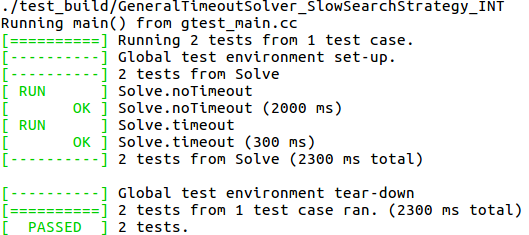
\includegraphics[width=0.9\textwidth]{Figures/google-test-output.png}
	\captionof{figure}{Google Test results from command line}
	\label{google-test-output}
\end{center}
The figure above\ref{google-test-output} was the output from \emph{GeneralTimeoutSolver\_SlowSearchStrategy\_INT} test suite. As the reader can see, the output from the test suite was the name of the test executed and if it passed the checks or not.  If a test does not pass the checks, the output becomes red, and the comparison which failed is printed. 
%----------------------------------------------------------------------------------------
%	BIBLIOGRAPHY
%----------------------------------------------------------------------------------------
\printbibliography[heading=bibintoc]
%\addcontentsline{toc}{chapter}{Bibliography}

%----------------------------------------------------------------------------------------

\end{document}  
